\clearpage 
\null 
\vfill 
\begin{center}
\textbf{\large Haizon Helet Cruz (42708)}
\end{center}
\vfill 
\fancyhead[L]{MNG Application (Haizon Helet Cruz 42708)}
\clearpage


\chapter{MNG Application Part I}
\section{THREAD SAFE RING BUFFER IMPLEMENTATION}
\subsection{Introduction}
The ring buffer or circular queue, is a storage mechanism designed to manage continuous streams of data within a fixed-memory footprint. This is unlike a linear queue which requires memory shifts or reallocation of elements are added and removed, a ring buffer connects its end back to its beginning. The choice of ring buffer, to be used in this project is fairly self explanatory, it is a very efficient operation particularly the enqueue and dequeue operations are performed in O(1) constant time, ensuring that the system’s throughput remains deterministic regardless of how much data has already been processed. 

In the context of Measurement Network Gateway, the ring buffer acts as a vital asynchronous bridge between two decoupled threads: the sensor data acquisition thread and network transmission thread. These threads are totally independent and without an appropriate storage mechanism will lead to catastrophic data loss. With the use of a ring buffer, the producer can “fire and forget” its data, while the consumer drains that data in optimized batches whenever the communication channel is ready. By encapsulating this logic with POSIX mutexes, the ring buffer ensures that even if both threads attempt to access the indices at the exact same time even down to a microsecond precision, its internal state remains consistent and memory-safe.

\subsection{ARCHITECTURAL ROLE IN MNG}
In the broader scope of the MNG architecture, the ring buffer serves as a temporal isolation layer, a critical bridge that decouples two threads with fundamentally incompatible timing characteristics. On the production side, the sensor acquisition thread operates within a hard real-time domain, requiring high-frequency, deterministic periodic sampling. This thread cannot afford to block or wait, as any delay would immediately violate real-time guarantees and destabilize the data’s temporal integrity. Conversely, the network streaming thread exists in an asynchronous, non-deterministic domain where it is subject to the unpredictable nature of TCP/IP congestion, signal jitter, and packet retransmissions.

Without the ring buffer acting as a mediator, the sensor task would be forced to inherit the network’s timing variability. If the network stalled, the sensor task would stall, leading to catastrophic failure in control loops. By implementing this module, the architecture enforces temporal decoupling, allowing the sensor thread to maintain its rigid sampling schedule regardless of the network's current state. The buffer effectively provides backpressure absorption, acting as a shock absorber that stores data during bursts of network congestion and drains it when bandwidth becomes available.

Ultimately, this design ensures a producer non-blocking guarantee. The sensor task can "fire and forget" its samples into the buffer with the assurance that the operation will always complete in O(1) time. This architectural role is finalized by ensuring data coherency under concurrency, where the mutex-protected FIFO queue allows these two disparate timing domains to exchange information safely. By transforming a chaotic, non-deterministic network demand into a structured, bounded memory operation, the ring buffer ensures the overall system remains stable, responsive, and accurate.

\subsection{DATA STRUCTURE DESIGN }
This section defines important factors considered during the implementation process of the said ring buffer:\\

\subsubsection*{Memory Determinism}
The ringBuffer was declared using the following piece of code referenced in \texttt{mainH.h}.
\begin{minted}[bgcolor = lightgray, tabsize = 4, breaklines]{c}
extern ring_buffer_t *rb;
\end{minted}

and its implementation was completed in \texttt{ringBuffer.c} and initialized in \texttt{main.c}.


\begin{figure}[H]
\centering 
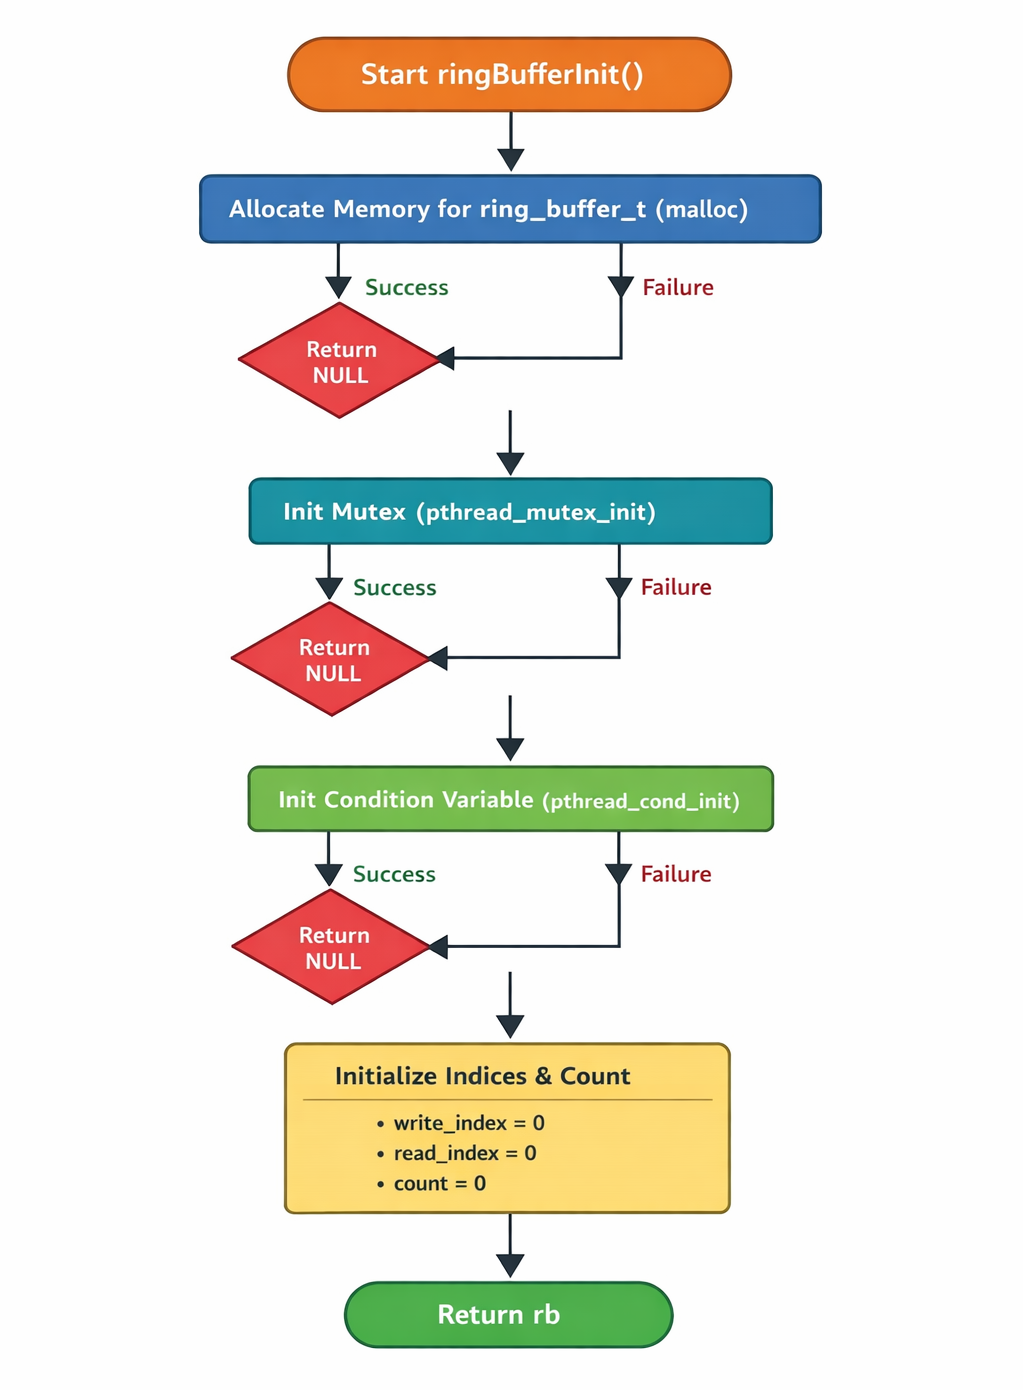
\includegraphics[scale = 0.35]{media/haizangui4.png}
\caption{Ring Buffer Data Init}
\label{fig-haizangui1}
\end{figure}

\clearpage 
\subsubsection*{Indexing Model}
The ring buffer type is defined using the following structure:

\begin{minted}[bgcolor = lightgray, tabsize = 4, breaklines]{c}
typedef struct ring_buffer
{
    pthread_mutex_t rbMutex;
    sensor_data_t sampleArray[RING_BUF_SIZE];
    size_t write_index;
    size_t read_index;
    uint16_t count;
    pthread_cond_t  data_available;
} ring_buffer_t;
\end{minted}
In the architecture of a circular buffer, the management of the \texttt{read\_index} and \texttt{write\_index} through modulo arithmetic is what enables the structure to simulate an infinite loop within a finite static memory block. By calculating the next position as \texttt{(index + 1)(mod N)}, the logic ensures that once the end of the buffer is reached, the pointer automatically wraps back to the zero-th index. This mathematical constraint is the key to the buffer’s O(1) efficiency.

Another logical challenge arises when using only \texttt{read\_index} and \texttt{write\_index} to determine the state of the buffer. In the implementation it becomes naive when the condition where \texttt{read\_index} and \texttt{write\_index} becomes equal, as the identical state occurs when the buffer is entirely empty and when it has been filled to its maximum capacity. To remove this ambiguity, we can use another variable named count. By maintaining a real time data count of the samples stored, the implementation can immediately disambiguate these states: if states are equal and the count is zero, the consumer knows there is nothing to process, whereas if they are equal and the count is N, the producer knows that the buffer is full and it must begin the overwrite procedure.

\subsection{Concurrency Model}
The concurrency model of the ring buffer is built upon the interaction between a producer thread, responsible for high-frequency sensor acquisition, and a consumer thread, which handles the non-deterministic timing of network transmissions. Because these two tasks operate asynchronously, they must access the same memory addresses for the sampleArray, indices, and count variable. This shared access necessitates the use of a POSIX mutex to enforce mutual exclusion, ensuring that only one thread can modify or evaluate the buffer’s internal state at any given microsecond. Without this lock, a race condition is nothing but certain when the producer updates the write\_index at the exact moment the consumer is attempting to read it, leading to “memory tearing” or a corrupted value of count.

Beyond simple mutual exclusion, the implementation utilizes a condition variable, data\_available, to manage the lifecycle of the consumer thread efficiently. Without such an implementation the consumer might “busy-wait”, constantly polling the buffer in a tight loop to see if new data has arrived, which needlessly consumes CPU cycles and increases power consumption. By integrating this condition, the consumer can instead enter a suspended state, relinquishing the processor until the producer explicitly signals that new data is ready. This transition from a “polling” model to a “signaled” model drastically reduces system overhead and ensures that the network task reacts with minimal latency the moment a sensor sample is successfully stored.

 In extension, the buffer following an overflow policy refers to the implementation decision to drop the oldest sample when the buffer reaches its maximum capacity, tailored for real-time telemetry systems. By advancing the read index in tandem with the write index during an overflow, the system effectively slides the window of available data forward. This ensures that the producer never encounters a block or wait state. In a streaming context, this non-blocking behavior is paramount; if the producer were forced to wait for a slow network consumer, the resulting sampling jitter would destabilize high-frequency control loops and cause the system’s real-time guarantees to collapse entirely.

\subsection{Insert Operation}
The insertion operation or addition of samples to the ring buffer is carried out using the function\\
\texttt{ringBufferAddSample} in \texttt{ringBuffer.c.}

The addition operation follows a strict, sequential protocol designed to maintain the integrity of the shared state while ensuring that the producer thread never experiences non-deterministic delays. By immediately acquiring the \texttt{rbMutex}, the function creates a protected critical section where the pointer arithmetic and the data write can occur without interference from the consumer thread. Once the \texttt{sensor\_data\_t }payload is copied into the sampleArray at current \texttt{write\_index}, the index is incremented using modulo arithmetic to facilitate the circular wrap-around.

The insertion logic rather than failing or blocking when the buffer is full, the function performs a conditional check on the count. If the ring buffer has reached \texttt{RING\_BUF\_SIZE}, the \texttt{read\_index} is manually advanced to the next position. This ensures that the \texttt{FIFO (First-IN-First-OUT)} order is preserved by effectively evicting the oldest sample to make room for the newest. Following the update of the indices and the count,  the function issues a \texttt{pthread\_cond\_signal} to the \texttt{data\_available} condition variable. This signal is essential for system efficiency, as it alerts any sleeping consumer thread that the buffer is no longer empty, transitioning the consumer from a suspended state back to an active processing state.

From a performance standpoint, the insertion operation is characterized by its O(1) constant time complexity. Because the implementation avoids heap interaction, dynamic resizing, or complex memory copying, the execution time remains identical whether the ring buffer is empty or nearly full. The lack of malloc or calloc calls within the write path is necessary for high-frequency sampling, as it eliminates the risk of non-deterministic latencies caused by memory management overhead or heap fragmentation. This makes the write path exceptionally reliable for real-time sensor tasks where every microsecond of jitter can impact the accuracy of the resulting data stream.

\subsection{Batch Extraction}
The extraction of samples in batch by the consumer or the network thread is done using the function \texttt{ringBufferRemoveBatch} in \texttt{ringBuffer.c}.

This function represents a critical performance optimization layer, moving beyond simple data retrieval to address the systemic overhead of concurrent execution. In a high-frequency environment, the cost of synchronization can often exceed the cost of data movement itself. Without a batching mechanism, extracting 100 samples would required 100 individual calls to a single-removal function, triggering 100 discrete lock and unlock cycles. Each cycle presents a fresh opportunity for the OS scheduler to perform a context switch, increasing the likelihood of mutex contention and causing significant cache invalidation as the processor repeatedly arbitrates into a single critical section, locking the mutex once to perform a linear memory transfer before releasing it.

Batching aligns perfectly with the requirements of network protocols. Since network hardware and TCP stacks operate most efficiently when handling larger payloads, the ability to drain the buffer in blocks allows the system to maximize packet utilization. This reduces the relative overhead of headers and improves overall bandwidth efficiency, ensuring that the network gateway remains a high-throughput conduit rather than a bottleneck. The function also ensures that the \texttt{read\_index} and count are updated in a single cohesive block after the target number of samples has been reached. This approach not only preserves the data structure invariants but also provides a deterministic execution path that is highly friendly to modern CPU instruction pipelining. In this gateway project, where sensor samples are processed fast, this batching strategy is not merely a convenience but a mandatory requirement for system stability. It transforms the read path into a high-speed data drain, ensuring the consumer can keep pace with a prolific producer while maintaining the lowest possible CPU overhead.

\begin{figure}[H]
\centering 
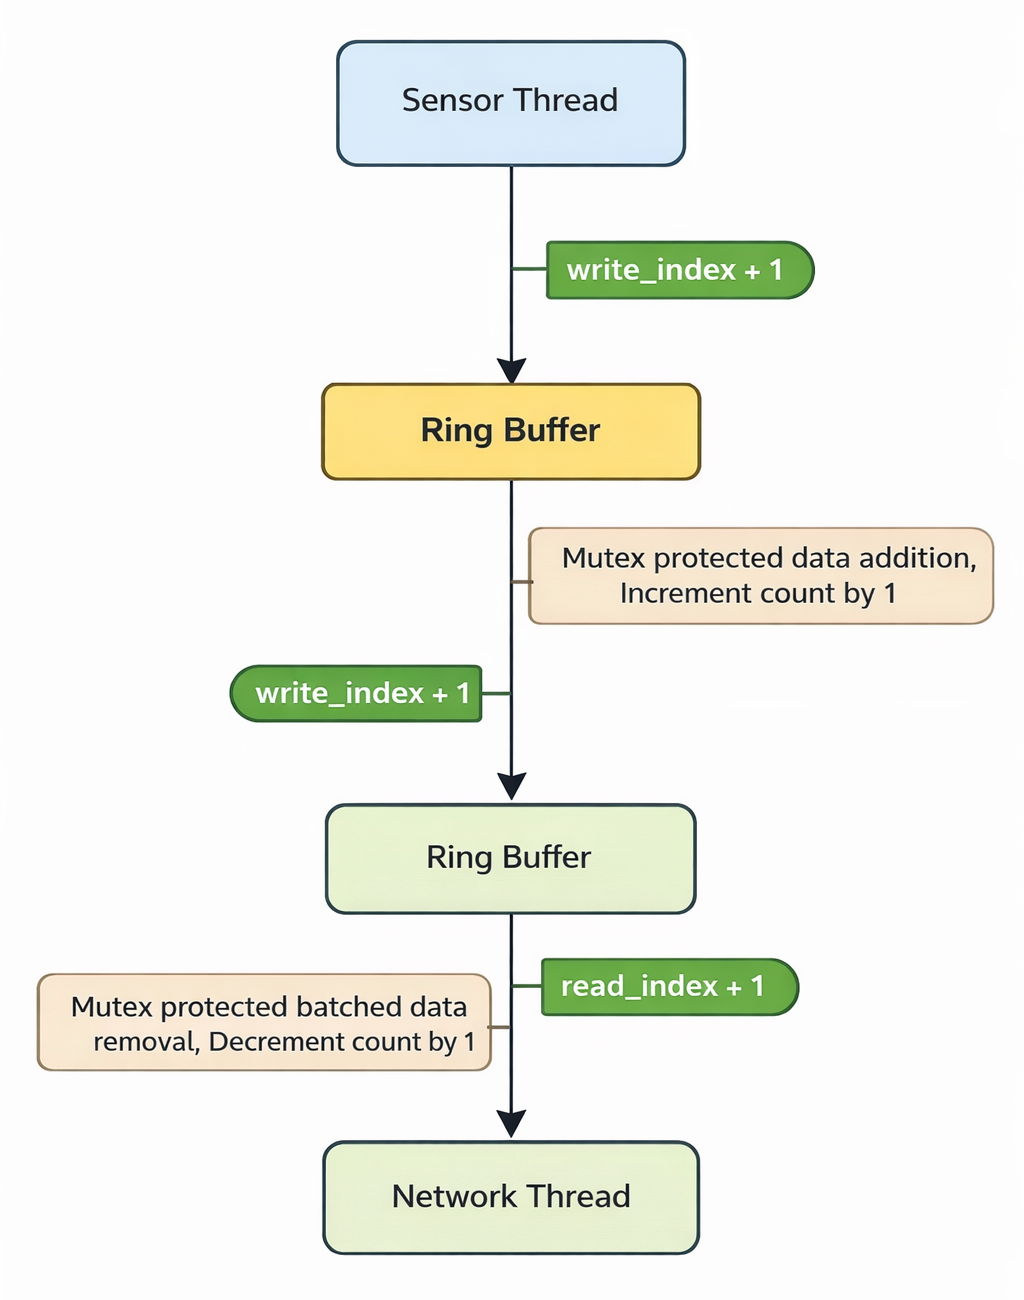
\includegraphics[scale = 0.24]{media/haizangui5.png}
\caption{Ring Buffer Data Flow}
\label{fig-haizangui2}
\end{figure}

\subsection{Complexity Analysis}
The efficiency of a ring buffer is best understood through a formal complexity analysis, which confirms that the design has reached the theoretical limit for queue based operations. Every core function-initialization, insertion, and both single and batch removal-operates within a deterministic time frame, regardless of the gateway’s uptime or the volume of data processed.

When the buffer is empty or requires an overwrite of the oldest sample, the operation involves a fixed number of index increments and a single memory copy which ensures O(1) complexity, while the batch remove function iterates through k samples, its complexity is technically O(k), however in the context of the data structure’s overhead, it remains optimal because it performs the minimum necessary work (one copy per element) while reducing the synchronization cost to O(1) per batch rather than O(k).

The space complexity of the insert method is O(N), where N is the \texttt{RING\_BUF\_SIZE}. This is the most efficient use of memory possible for a buffer, as it allocates exactly enough space for the required data without any hidden pointers, metadata nodes, or dynamic overhead associated with linked-list implementations. Because the memory is statically defined within the \texttt{ring\_buffer\_t} struct, the system’s memory footprint is entirely predictable at compile-time, which is a prerequisite for safety-critical embedded applications.

Beyond the standard Big O notation, the implementation is optimized for real-time determinism. By avoiding heap-based functions like malloc() and free() during the write and read paths, the code eliminates the risk of “Long-Tail latency” caused by memory fragmentation or garbage collection cycles. The use of a single mutex ensures that while the threads are synchronized, the “lock-time” remains minimal and constant. This makes the ring buffer an “optimal” bridge: it provides the highest possible throughput with the lowest possible jitter, satisfying the rigorous timing constraints of high-frequency sensor acquisition and network streaming.

\begin{table}[H]
    \centering 
        \begin{tabular}{lll}
        \toprule
		\textbf{Operation} & \textbf{Time Complexity} & \textbf{Space Complexity} \\
		\midrule 
		Insert & $O(1)$ & $O(N)$ fixed \\
		Batch Remove &  $O(k)$ & $O(1)$ \\
        \bottomrule
    \end{tabular}
\end{table}

where: \\
N = 2048, \\
K = number of samples extracted in a batch. \\

The size of the ring buffer was decided on the following calculation\\
Max sampling rate = 1kHz, and a network stall of 2 seconds. 


This means the need is 2000 samples, Buffer sizing is derived from the calculation that the size should be greater than or equal to the product of sampling frequency and network stall time.


\subsection{Summary}
The ringBuffer module is bounded, mutex-protected circular FIFO designed to provide deterministic temporal decoupling between a real-time sensor acquisition thread and a non-deterministic network transmission thread. It uses static memory allocation to guarantee runtime predictability and eliminate fragmentation, constant-time index arithmetic to avoid data movement, and a lossy overwrite strategy to preserve sampling determinism under overflow conditions. Batch extraction minimizes synchronization overhead and improves network throughput efficiency.


\clearpage 
\section{COMMUNICATION NETWORK IMPLEMENTATION}
This chapter provides a detailed technical analysis of the network thread implementation (\texttt{networkThread.c}). This section focuses on the MNG’s communication gateway, utilizing the Berkeley Sockets API to provide a high performance, command driven TCP server. It is specially engineered to bridge the gap between internal data structures and external clients, ensuring that sensor data is delivered with minimal latency and high reliability. The use of a separate thread for the purpose of client communication to server, isolates the data acquisition thread thus providing continuous data transfer.


\subsection{SOCKET CREATION}
The initialization phase of \texttt{networkThread.c} establishes the foundation for reliable communication using the TCP \texttt{(SOCK\_STREAM)} protocol. The process begins by creating a file descriptor using the socket() system call, followed immediately by setting the \texttt{SO\_REUSEADDR} option via \texttt{setsockopt()}. This is a critical step for high-availability systems, as it allows the server to bind to the same port without waiting for the kernel’s protocol timeout after a restart.

The server configuration utilizes the \texttt{sockaddr\_in} structure, binding to \texttt{INADDR\_ANY} to allow connections from any network interface on the host. By executing bind() and listen(), the thread transitions the socket into a passive state, ready to queue incoming connection requests. This setup ensures that the communication gateway is isolated and ready to serve data before entering its main execution loop.

\subsection{STATE MACHINE IMPLEMENTATION}
The state machine represents different states in the whole lifecycle of the network thread. There are three main states:
\begin{itemize}
\item STREAM\_IDLE
\item STREAM\_RUNNING
\item STREAM\_DISCONNECT
\end{itemize}

These states are defined as enums shown below:
\begin{minted}[bgcolor = lightgray, tabsize = 4, breaklines]{c}
typedef enum
{
   STREAM_IDLE,
   STREAM_RUNNING,
   STREAM_DISCONNECT
} stream_t;
\end{minted}

\begin{figure}[H]
\centering 
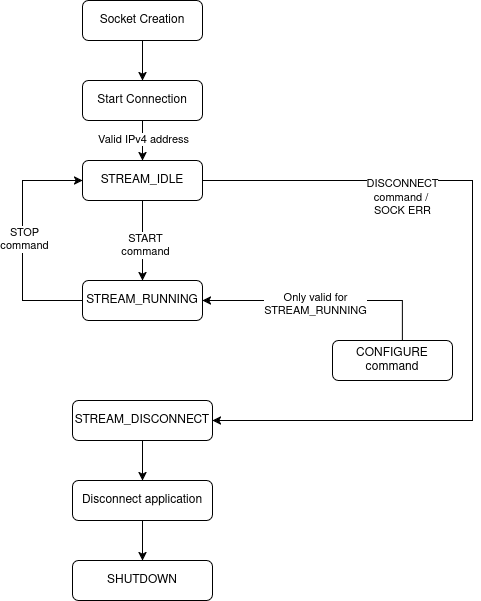
\includegraphics[scale = 0.5]{media/haizangui3.png}
\caption{Socket Creation}
\label{fig-haizangui3}
\end{figure}

\textbf{STREAM\_IDLE STATE}\\
This state represents the state where the application layer has made a successful connection with the GUI but the data is not streaming and the configuration commands are not applied. As the name suggests this is the idle state where the system remains connected.\\

\textbf{STREAM\_RUNNING STATE}\\
This state represents where the application layer is actively streaming data to the GUI and is ready to receive configuration commands from the GUI. This state is activated when the server receives the “START” command from the client side. The main action involved in this state is draining the ring buffer using the function \texttt{ringBufferRemoveBatch}, and then sending the payload in batches, to ensure proper use of TCP frames in the Ethernet connection.\\

To ensure data integrity and proper framing over a stream-oriented TCP connection, the implementation uses a length-prefixing technique. The server first calculates the total payload size, converts it to network byte order using htonl(), and sends this 4-byte header. Only after the header is successfully sent does it transmit the actual sensor data payload. The use of while loop around the send() calls accounts for partial writes, ensuring that every byte of the batch is delivered. If a transmission error occurs, the state machine transitions to \texttt{STREAM\_DISCONNECT}, where it gracefully shutdown the socket and releases resources to prevent memory leaks or hanging connections.\\

\textbf{STREAM\_DISCONNECT STATE}\\
Stream disconnect state is the state when the application layer has received the shutdown command and should kill the process. This is different from the idle state because it only shuts down connection with the client. This state represents the entire MNG application is offline.

\begin{minted}[bgcolor = lightgray, tabsize = 4, breaklines]{c}
if (stream_state == STREAM_DISCONNECT)
{
  printf("Closing client connection...\n");
  shutdown(client_fd, SHUT_RDWR);
  close(client_fd);
  break;
}
\end{minted}



\subsection{CONFIGURATION COMMANDS}
The network thread features an integrated command parser that allows external clients to dynamically control the MNG’s behavior. Upon receiving the data via recv(), the server sanitizes the input by stripping newline characters and comparing the string against a predefined command set. This allows for real-time state transactions, such as switching between \texttt{STREAM\_IDLE, STREAM\_RUNNING, STREAM\_DISCONNECT.}\\

\textbf{CONNECT COMMAND}\\
The connect command is for the socket connection between the application layer and the GUI. This command sends the IPv4 address which is used to connect. Only valid IPv4 address is used and hence required validation has been added in the GUI. \\


\textbf{START COMMAND}\\
The purpose of this command is to transfer the application from \texttt{STREAM\_IDLE} to \texttt{STREAM\_RUNNING} state, this will make the network layer drain the ring buffer and start sending the data in batches to the client. The START command is only valid if the application layer is connected and is not already streaming data to the GUI. Therefore required validation has been added in the GUI. 
\begin{minted}[bgcolor = lightgray, tabsize = 4, breaklines]{c}
if (!strcmp(cmd_buffer, "START"))
 {
    stream_state = STREAM_RUNNING;
 }
\end{minted}
\smallskip


\textbf{CONFIGURE COMMAND}\\
A significant feature of this section is the CONFIGURE command, which allows for live updates to individual sensor sampling rates. By parsing the command string with \texttt{sscanf()}, the server identifies the specific sensor and desired frequency in Hz. To maintain thread safety, the implementation utilizes POSIX mutexes (\texttt{pthread\_mutex\_lock}), ensuring that updating the \texttt{rate\_hz} and \texttt{period\_us} values does not create race conditions with the data acquisition thread. This architecture provides a clear separation of concerts: while the acquisition thread remains focused on high-speed sampling, the network thread provides a safe, low-latency interface for remote management and system shutdown. CONFIGURE command is only valid during STREAM\_RUNNING state and hence the required validation has been added to the GUI. 

\begin{minted}[bgcolor = lightgray, tabsize = 4, breaklines]{c}
if (!strncmp(cmd_buffer, "CONFIGURE", 9))
   {
       char sensor[16];
       uint32_t rate;

       if (sscanf(cmd_buffer, "CONFIGURE %15s %u", sensor, &rate) == 2)
       {
           int sid = sensor_from_string(sensor);
           if (sid >= 0 && rate > 0)
           {
               pthread_mutex_lock(&sensor_cfg[sid].lock);
               sensor_cfg[sid].rate_hz = rate;
               sensor_cfg[sid].period_us = 1000000ULL / rate;
               sensor_cfg[sid].next_deadline = getElapsedTime() + 
                                              sensor_cfg[sid].period_us;
               pthread_mutex_unlock(&sensor_cfg[sid].lock);
               printf("[SERVER] CONFIGURE applied\n");
           }
       }
   }
\end{minted}
\smallskip

\textbf{STOP COMMAND}\\
The stop command is used to send instructions to the application layer to stop streaming data to the GUI, while maintaining the connection. STOP command is only valid when the application layer was already streaming, hence such a validation is applied in the GUI. 

\begin{minted}[bgcolor = lightgray, tabsize = 4, breaklines]{c}
if (!strcmp(cmd_buffer, "STOP"))
{
  stream_state = STREAM_IDLE;
}
\end{minted}
\smallskip

\textbf{DISCONNECT COMMAND}\\
The disconnect command is used to disconnect the socket from the GUI. This is different from the IDLE state as the application and GUI are no longer connected. This command is only valid if the application layer and GUI are already connected via a valid IPv4 address and cannot be disconnected if the application layer is already streaming. The user will have to stop the streaming using STOP command first and then use DISCONNECT to cut the connection, and hence required validation has been added in the GUI.
\begin{minted}[bgcolor = lightgray, tabsize = 4, breaklines]{c}
if (!strcmp(cmd_buffer, "DISCONNECT"))
{
  stream_state = STREAM_DISCONNECT;
}
\end{minted}
\smallskip

\textbf{SHUTDOWN COMMAND}\\
Shutdown command is used to shutdown the whole application by setting the global variable system\_running to 0. This will clear all resources allocated and put the system to rest. 
\begin{minted}[bgcolor = lightgray, tabsize = 4, breaklines]{c}
if (!strcmp(cmd_buffer, "SHUTDOWN"))
{
  printf("Shutting down...\n");
  system_running = 0;
  stream_state = STREAM_DISCONNECT;
}
\end{minted}
\smallskip

\clearpage
\subsection{CONCLUSION}
The \texttt{networkThread.c} implementation delivers a structured, robust, and production-oriented communication layer for the Measurement Network Gateway. By isolating TCP communication within a dedicated thread, the design prevents network latency or client-side delays from interfering with deterministic sensor acquisition. This separation is not just architectural cleanliness — it is essential for maintaining real-time performance and system stability.

The use of a well-defined state machine \texttt{(STREAM\_IDLE, STREAM\_RUNNING, STREAM\_DISCONNECT)} ensures predictable behavior across the entire lifecycle of the connection. Explicit state transitions eliminate ambiguity, reduce unintended side effects, and simplify debugging. The implementation of length-prefixed TCP framing, combined with guarded \texttt{send()} loops, demonstrates careful handling of stream-oriented communication and partial writes a critical detail often overlooked in simpler designs.
Dynamic runtime configuration through structured command parsing enables flexibility without compromising thread safety. The use of POSIX mutexes to protect shared sensor parameters prevents race conditions, reinforcing the reliability of concurrent operations. Additionally, graceful shutdown handling ensures proper resource cleanup and prevents socket or memory leaks.
Overall, the module provides a reliable, low-latency, and extensible TCP server architecture capable of supporting real-time streaming and remote configuration. Its design reflects strong attention to concurrency control, communication integrity, and system resilience all essential characteristics of a well-engineed embedded networking solution.

\clearpage 
\null 
\vfill 
\begin{center}
\textbf{\large Alin Raj Rajagopalan Nair (41520)}
\end{center}
\vfill 
\fancyhead[L]{MNG Application (Alin Raj Rajagopalan Nair 41520)}
\clearpage

\chapter{MNG Application part II}
\section{MAX31865}
\subsection{Temperature Conversion}
Sensors that change resistance in response to temperature are known as
resistance temperature detectors (RTDs). Platinum RTDs, also known as
PT-RTDs, are the most widely used and precise wire material. RTDs can
also be made of copper, nickel, and other metals. Platinum RTDs provide
good accuracy and repeatability, decent linearity, and a broad
temperature range (to above +800NC). Although there are additional
numbers available, 100I and 1kI are the most often used nominal
resistance levels for PT-RTDs at 0NC. Alpha (α) is the average slope
between 0NC and +100NC. The contaminants and their concentrations in the
platinum determine this value. The two most commonly used alpha values,
which correspond to the SAMA and IEC 751 (PT100) standards, are 0.00385
and 0.00392 temperature Conversion.

Based on this the resistance vs temperature graph is almost linear , but
at some points the curvature exists as mentioned in the ~Callendar- Van
Dusen equation:

\begin{align*}
R(T) = R_0 \cdot (1 + aT + bT^2 +c \cdot (T - 100) T^3)
\end{align*}

where: 

$T$: Temperature (\unit{\degreeCelsius})\\
$R(T)$: resistance at T \\ 
$R_0$: resistance at $T = \SI{0}{\degreeCelsius}$\\ 
$\alpha$: 0.00385055 is specified in the IEC 751\\ 
The following are the Callender-Van Dusen coefficient values: 
$a = 3.90830 \times 10^{-3}$\\
$b = -5.77500 \times 10^{-7}$\\ 
$c = -4.18301 \times 10^{-12}$ for $-200 \unit{\degreeCelsius} \leq T \leq 0 \unit{\degreeCelsius}$, 0 for $0 \unit{\degreeCelsius} \leq T + 850 \unit{\degreeCelsius}$ 
Figure illustrates that the resistance of a PT100 RTD increases with
temperature in a slightly nonlinear manner, following the standardized
platinum resistance--temperature relationship. For practical purposes
within the 0 \unit{\degreeCelsius} to 100 \unit{\degreeCelsius} range, this characteristic can be approximated
by a straight line with a slope of approximately 0.385 \unit{\ohm}/\unit{\degreeCelsius}, which
simplifies calculations while introducing only minimal deviation from
the actual curve.

\begin{figure}[H]
\centering 
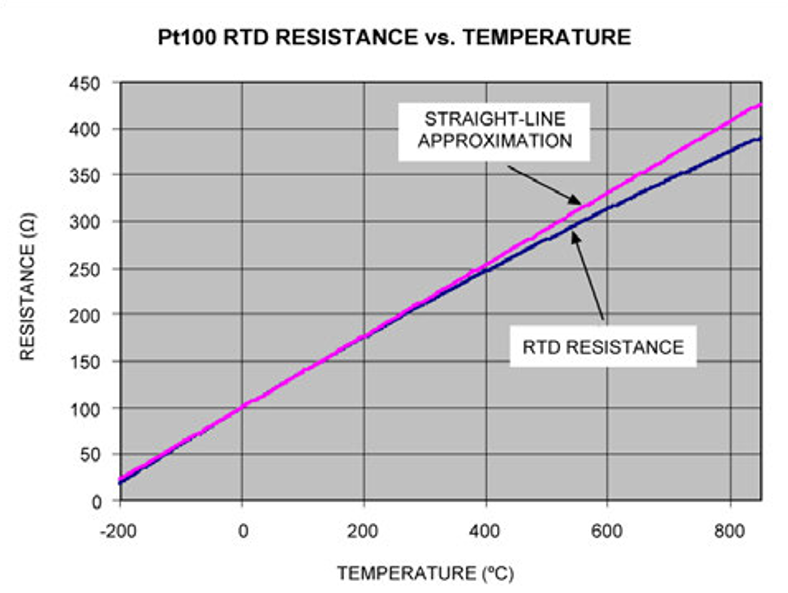
\includegraphics[width = 0.6\textwidth]{media/alin1.png}
\caption{PT100 RTD Resistance vs Temperature}
\label{fig-alin1}
\end{figure}

\subsection{Typical Application Circuits}
There are 3 ways in which we can typically measure the resistance and
they are listed as follows

\begin{enumerate}
\item 2-Wire Measurement: In a 2-wire configuration, the same pair of conductors is used both to supply the excitation current and to sense the voltage across the RTD, which means the resistance of the lead wires is directly added to the sensor resistance. 
For a PT100, whose sensitivity is approximately 0.385 \unit{\ohm / \degreeCelsius}, an additional series 
resistance of 0.4 \unit{\ohm} corresponds to a temperature error of about 1 \unit{\degreeCelsius} (0.4 \unit{\ohm} ÷ 0.385 \unit{\ohm / \degreeCelsius} $\approx$ 1 \unit{\degreeCelsius}). While this error may be negligible when the RTD is mounted very close 
to the MAX31865 and the lead length is short, the resistance of longer cables increases proportionally with length and conductor size, causing a systematic positive temperature to offset. Consequently, in installations with extended wiring, the accumulated lead resistance can introduce significant measurement inaccuracies, making 3-wire or 4-wire configurations preferable for improved compensation and precision.

\begin{figure}[H]
 \centering 
 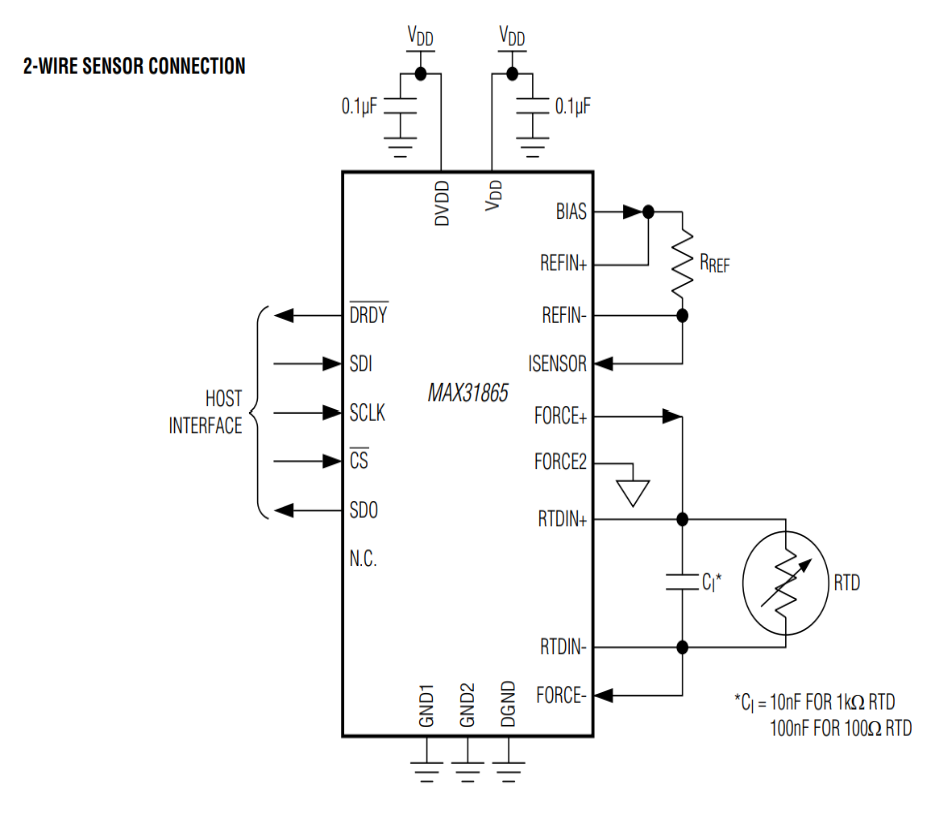
\includegraphics[scale = 1]{media/alin2b.png}
 \caption{Wire Sensor Connection circuit}
 \label{fig-alin2}
 \end{figure} 
 
 
 
\item 3-Wire Measurement: In a 3-wire configuration, two conductors are connected to one side of the RTD element and a third conductor is connected to the opposite side, allowing partial compensation of lead resistance while using fewer wires than a full 4-wire (Kelvin) setup. The MAX31865 applies a precise excitation current through the RTD and measures two voltages: the voltage across the RTD terminals (RTDIN+ to RTDIN−) and the voltage drop across the current-carrying return lead (via the FORCE2 sampling input). By subtracting the measured lead voltage from the total sensed voltage, the device effectively removes the contribution of one lead resistance from the calculation.

      This compensation method assumes that the two current-carrying leads have approximately equal resistance; when they are well matched in length and cross-section, their voltage drops are nearly identical and cancel each other, significantly reducing measurement error. Although a small residual error may remain if the lead resistances are unequal or subject to temperature gradients, the 3-wire approach provides a practical balance between wiring complexity and measurement accuracy, making it the most widely used configuration in industrial PT100 applications.

\begin{figure}[H]
\centering 
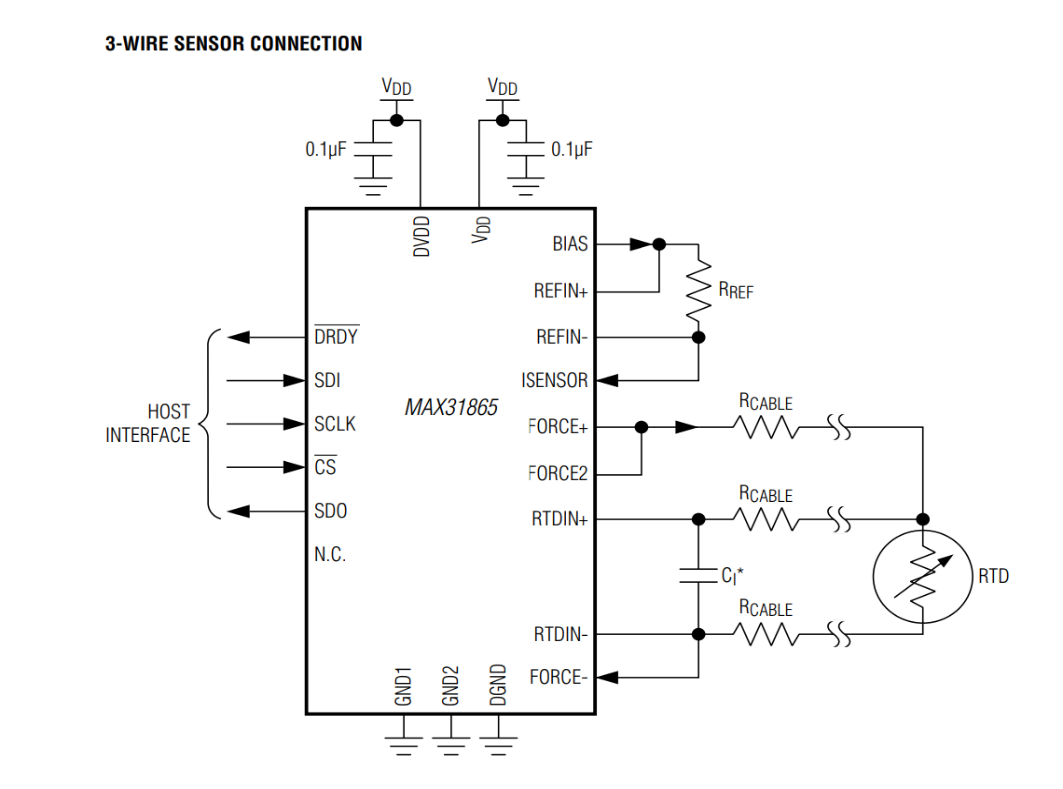
\includegraphics[scale = 1]{media/alin3.png}
\caption{3-Wire Sensor Connection}
\label{fig-alin3}
\end{figure}

\item 	4-Wire Measurement: The 4-wire connection eliminates errors due to cable resistance by using two conductors to supply the excitation (force) current and two separate conductors to sense the voltage directly across the RTD element. Because the sense inputs draw negligible current, virtually no voltage drop occurs along the sense leads, meaning the measured voltage reflects only the true RTD resistance and not the resistance of the connecting wires. As a result, the calculated resistance
 ( $R=V/I$ ) is independent of cable length and lead resistance, providing the highest possible measurement accuracy, particularly in applications with long cable runs or where precise temperature determination is required.
 
 \begin{figure}[H]
 \centering 
 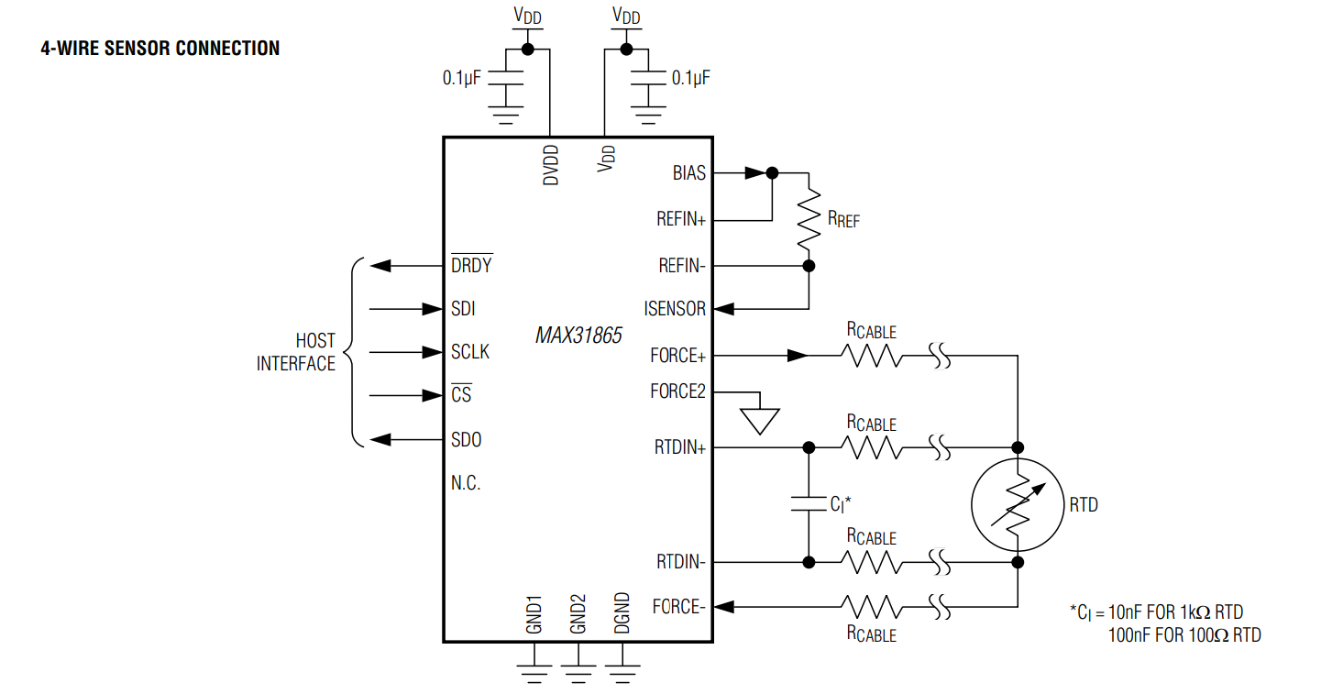
\includegraphics[scale = 1]{media/alin4.png}
 \caption{4-Wire Sensor Connection circuit}
 \label{fig-alin4}
 \end{figure}
\end{enumerate}

\section{Internal Registers}
\subsection{Introduction}
The MAX31865 is a precision RTD-to-digital converter designed to interface platinum RTDs such as PT100 and PT1000 with a microcontroller via an SPI interface. It integrates a precision bias current source, a 15-bit sigma-delta ADC, fault detection circuitry, and digital filtering. All device configuration, measurement data, and diagnostic information are accessed through a small set of internal registers. These registers allow the user to control operating modes, read conversion results, define fault thresholds, and monitor system integrity. 
The registers are accessed using the 0Xh addresses for reads and the 8Xh addresses for writes. Data is read from or written to the registers MSB first.
\begin{figure}[H]
\centering 
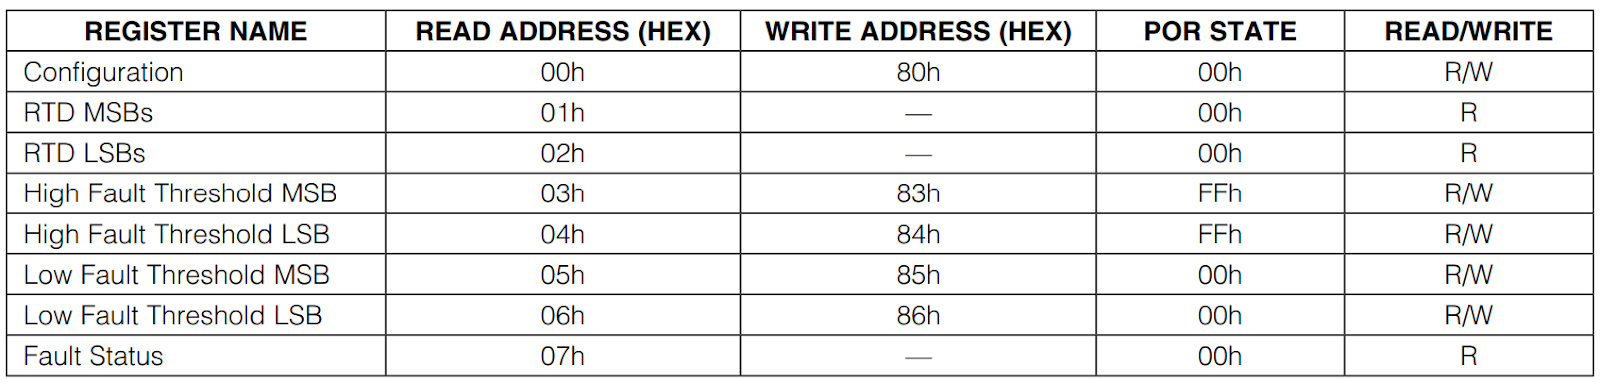
\includegraphics[width = \textwidth]{media/alin2.png}
\caption{Internal registers of MAX31865}
\label{fig-alin2bc}
\end{figure}

\subsection{Configuration Registers (00h)}
The Configuration Register (address 00h) is an 8-bit control register that determines the complete operating behaviour of the MAX31865. It governs excitation control, ADC conversion timing, wiring compensation, fault detection routines, and digital noise filtering. Since the MAX31865 performs ratio-metric resistance measurement using a precision reference resistor, correct initialization of this register is essential for stable and accurate RTD measurements.

\textbf{Operational Control and Measurement Modes}
One of the primary functions of this register is to control how conversions are executed. The device can operate in:

\begin{itemize}
\item Continuous (automatic) conversion mode, where the sigma-delta ADC continuously updates the RTD data registers at fixed intervals. This mode is suitable for real-time temperature monitoring systems.
\item Normally-off mode, where the ADC remains idle until a 1-shot conversion is triggered. This approach reduces power consumption and minimizes RTD self-heating, which is particularly important in precision or battery-powered applications.
\end{itemize}
The 1-shot control bit initiates a single conversion cycle and automatically clears once the conversion is complete.

\begin{figure}[H]
\centering 
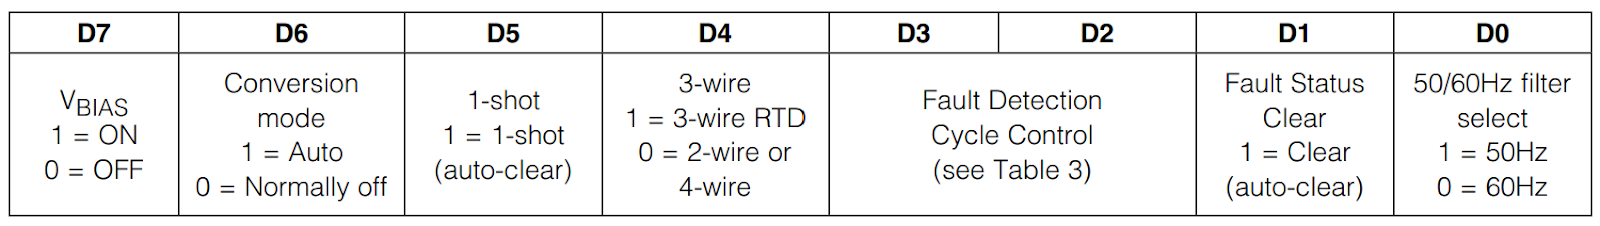
\includegraphics[width = \textwidth]{media/alin5.png}
\caption{Configuration register of MAX31865}
\label{fig-}
\end{figure}

\subsubsection{BIAS (D7)}
The configuration register controls the activation of the internal bias voltage (VBIAS), which provides the excitation current required for RTD measurement. When VBIAS is enabled, a controlled current flows through both the RTD and the precision reference resistor, allowing the ADC to measure the ratio of their voltages and accurately determine the RTD resistance. However, if no conversion is being performed, VBIAS can be disabled to stop the excitation current, thereby reducing power dissipation, minimizing sensor self-heating effects, and limiting long-term thermal drift.

In single (1-shot) conversion mode, it is good practice to set the VBIAS bit to ‘1’ shortly before initiating a conversion, allow a brief stabilization time, and then trigger the measurement. After the conversion is complete, VBIAS may be cleared again to conserve energy and maintain measurement accuracy. In contrast, when automatic (continuous) conversion mode is selected, the bias voltage remains enabled continuously to support uninterrupted ADC operation and real-time temperature monitoring.

\subsubsection{Conversion Mode (D6)}
The Conversion Mode bit in the configuration register determines whether the MAX31865 operates in continuous measurement mode or in normally-off (manual) mode. When this bit is set to ‘1’, the device enters automatic conversion mode, in which the internal sigma-delta ADC performs conversions continuously at a rate synchronized with the selected 50 Hz or 60 Hz digital filter. In this mode, new RTD data is updated automatically at regular intervals, making it suitable for real-time temperature monitoring applications where continuous measurement is required.

When the bit is cleared to ‘0’, the device exits automatic mode and enters Normally Off mode, in which no conversions are performed unless explicitly commanded. This mode is commonly used in low-power or precision systems to reduce energy consumption and minimize RTD self-heating. While in Normally Off mode, a single measurement can be initiated by setting the 1-shot bit, which triggers one complete conversion cycle. After the conversion is finished, the ADC returns to the idle state until another 1-shot command is issued.

Thus, the Conversion Mode bit allows the user to select between continuous real-time measurement and controlled, on-demand conversion depending on system requirements for power efficiency and measurement frequency.

\subsubsection{Shot-bit (D5)}
The 1-Shot bit (D5) is used to initiate a single resistance conversion when the device is operating in Normally Off mode (i.e., when the Conversion Mode bit is set to ‘0’). Writing a logic ‘1’ to this bit commands the MAX31865 to perform one complete ADC conversion cycle. The actual conversion process begins when the SPI transaction ends and the CS (Chip Select) line transitions high after the bit has been written.

Once triggered, the device performs a full resistance measurement using the selected digital filter setting. The conversion time depends on the chosen mains rejection filter:
\begin{itemize}
\item Approximately 52 ms when the 60 Hz filter is selected
\item Approximately 62.5 ms when the 50 Hz filter is selected
\end{itemize}

The longer duration in 50 Hz mode is due to the digital filtering process, which integrates over one full mains cycle to effectively suppress line-frequency noise.

The 1-Shot bit is self-clearing, meaning it automatically returns to ‘0’ once the conversion has started. This ensures that only a single measurement cycle is executed per command and prevents unintended repeated conversions. After completion, the ADC result is stored in the RTD data registers, and the device returns to the idle state until another 1-Shot command is issued.
This feature is particularly useful in low-power applications, where measurements are taken periodically rather than continuously, helping to minimize power consumption and RTD self-heating effects.

\subsubsection{bit (D4)}
The 3-Wire bit (D4) configures the MAX31865 for use with a 3-wire RTD connection. When this bit is set to ‘1’, the device activates its internal lead-resistance compensation circuitry. In this configuration, the MAX31865 measures the voltage between FORCE+ and RTDIN+ and subtracts it from the total measured voltage (RTDIN+ − RTDIN−). This subtraction compensates for the voltage drop (I·R drop) that occurs along the shared return lead, which carries both excitation current and sense current in a 3-wire arrangement.

The compensation method assumes that the two current-carrying leads have approximately equal resistance. When the lead resistances are well matched, the IR errors introduced by cable resistance are effectively cancelled, significantly improving measurement accuracy compared to a 2-wire configuration. However, if the lead resistances differ due to unequal cable lengths or temperature gradients, a small residual error may remain.

When using either a 2-wire or 4-wire RTD configuration, this bit must be written as ‘0’, disabling the internal 3-wire compensation circuitry and ensuring correct measurement operation for those wiring modes. Proper setting of the 3-Wire bit is essential to avoid incorrect resistance calculations and measurement inaccuracies.


\subsubsection{Fault Detection Cycle Bits (D3:D2)}
The Fault Detection Cycle bits (D3:D2) control the execution of the master-initiated diagnostic routine within the MAX31865. This routine is used to detect wiring faults and abnormal operating conditions such as open-circuit RTDs, short circuits, reference resistor faults, and overvoltage or undervoltage conditions. The fault detection mechanism applies specific internal test conditions to the RTD inputs and evaluates the resulting signals to determine whether a fault exists.

The fault detection cycle can operate in automatic timing mode or manual timing mode. In automatic mode, the device internally manages the timing sequence of the diagnostic procedure. The user only initiates the cycle, and the MAX31865 completes the test according to its predefined internal timing intervals. This mode is suitable for standard applications where no significant external filtering affects signal response.

In contrast, manual mode timing allows the system controller (microcontroller) to manage the timing steps of the fault detection process. This is particularly important when the external RTD interface circuitry includes additional input filtering components with a time constant greater than approximately 100 µs. Large time constants slow the settling of voltages during diagnostic testing, and automatic timing may not allow sufficient time for signals to stabilize. In such cases, manual control ensures accurate fault detection by providing adequate settling time between test phases.

Therefore, the selection between automatic and manual fault detection timing depends on the external analog filtering characteristics and overall system design requirements.

\subsubsection{Fault Status Clear Bit (D1)}
The Fault Status Clear bit (D1) is used to reset all latched fault indicators stored in the Fault Status Register. To properly clear the fault flags, a logic ‘1’ must be written to D1 while simultaneously ensuring that bits D5 (1-Shot) and D3:D2 (Fault Detection Cycle) are written as ‘0’. When this condition is met, all fault status bits D[7:2] in the Fault Status Register are cleared and returned to ‘0’.

It is important to note that clearing the fault register does not remove the actual fault condition from the system. If the underlying issue—such as an overvoltage or undervoltage condition—still exists, the corresponding fault bit (specifically bit D2 in the Fault Status Register) may be set again immediately after the reset operation. Consequently, the fault indicator bit in the RTD LSB register (D0) may also be reasserted if the fault persists.

The Fault Status Clear bit is self-clearing, meaning it automatically returns to ‘0’ after the clearing operation is completed. This ensures that the reset action occurs only once per command and prevents unintended repeated clearing of diagnostic flags.

\subsubsection{50/60 Hz Filter Select Bit (D0)}
The 50/60 Hz bit (D0) selects the notch frequency of the internal digital noise rejection filter in the MAX31865. This filter is designed to suppress interference from mains power frequencies that can couple into the RTD wiring and affect measurement accuracy. Since industrial and laboratory environments often contain electromagnetic noise at the local power-line frequency, proper selection of this bit significantly improves measurement stability.

When D0 = 0, the device configures its digital filter to reject 60 Hz and its harmonic components. This setting is typically used in regions where the mains supply frequency is 60 Hz. Conversely, when D0 = 1, the filter is configured to reject 50 Hz and its harmonics, which is appropriate for regions operating on a 50 Hz power grid.

The filter works by synchronizing the ADC integration time with the selected mains frequency, effectively averaging out periodic noise components. As a result, selecting the correct notch frequency reduces ripple, improves signal stability, and enhances overall temperature measurement accuracy in electrically noisy environments.

\subsubsection{RTD Resistance Registers (01h–02h)}
The RTD Resistance Registers (addresses 01h and 02h) store the digital conversion result of the measured RTD resistance. These consist of two 8-bit registers: the RTD MSB register (01h) and the RTD LSB register (02h). Together, they form a 16-bit word in which the upper 15 bits represent the measured resistance value, while the least significant bit (D0 of the LSB register) serves as a fault indicator.

The measurement result is expressed as a 15-bit ratio of the RTD resistance to the external reference resistor resistance. Internally, the MAX31865 performs a ratio metric measurement using its sigma-delta ADC, comparing the voltage drop across the RTD to the voltage across the precision reference resistor. The resulting digital code corresponds to:\\

ADC code = $R_{RTD} / R_{REF} \cdot 2^15$ \\ 
To calculate the actual RTD resistance, the following relationship is used:\\

$R_{RTD} = (ADC\ code / 32768) \cdot R_{REF}$\\

where 32768 represents the full-scale value of the 15-bit ADC.

Bit D0 of the RTD LSB register is reserved as a Fault flag. If this bit is set to ‘1’, it indicates that a fault condition has been detected, and the system should check the Fault Status Register (07h) to determine the specific cause.

These registers provide the primary measurement data required for temperature calculation and are read by the microcontroller after each completed conversion. 

\begin{figure}[H]
\centering 
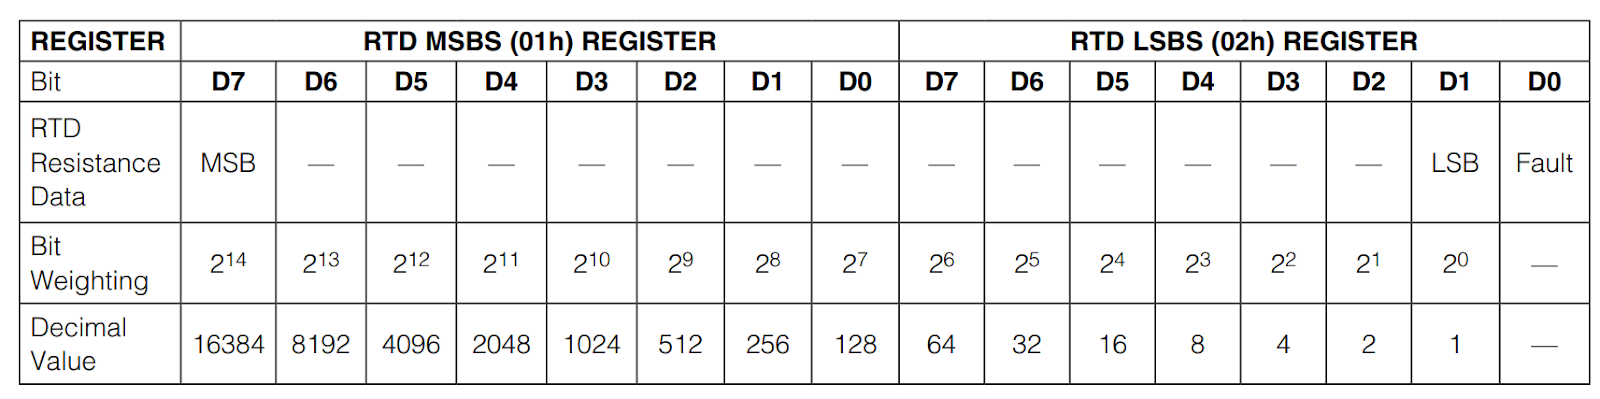
\includegraphics[width = \textwidth]{media/alin6.png}
\caption{RTD Resistance register layout}
\label{fig-alin6}
\end{figure}

\section{Types of Operation}
\subsection{Writing to MAX31865 registers (writeMAXSpiInterface())}
To write to any register in the MAX31865, the function writeMAXSpiInterface() is used. This function constructs a 16-bit SPI data frame where the Most Significant Byte (MSB 8 bits, bit 15 to 8) contains the register address with the write bit set, and the Least Significant Byte (LSB 8 bits, bit 7 to 0) contains the data value to be written. Every MAX31865 register has one read address and one write address [if the register is read-only, then writing to it does not affect its contents].\\

write address = read address | 0x80\\

example: writing 0xA1 in configuration register
read address of configuration register is 0x00 so its write address becomes 0x80.\\

MSB 8 bits (15 to 8) becomes 0x80 and LSB 8 bits (7 to 0) becomes 0xA1. so the whole data frame becomes 0x80A1. Writing this data frame to the kernel module register via \\ 

\textbf{\texttt{write(fd, \&tf\_obj\_snd, MEASOBJ\_SIZE);}}\\
will initiate the SPI communication.
The function then polls the status register by checking bit 0. When the status bit becomes 1, the SPI transaction is complete.
For writing to MAX31865, the function 
\begin{figure}[H]
\centering 
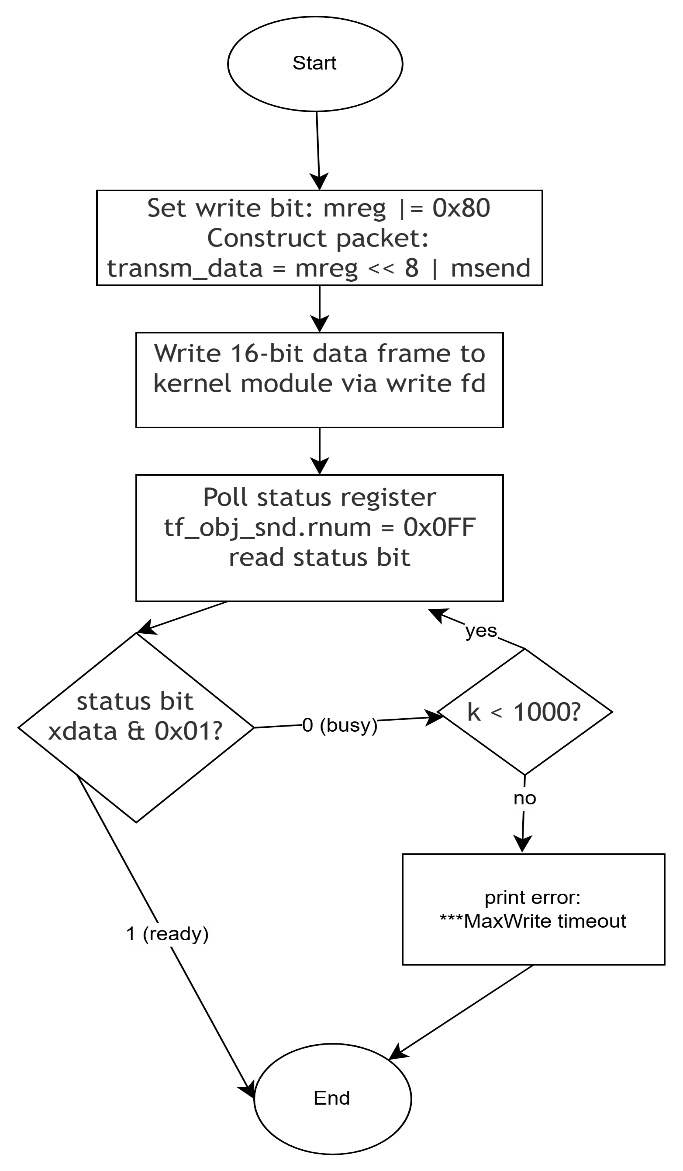
\includegraphics[scale = 1]{media/alin7.png}
\caption{write algorithm}
\label{fig-}
\end{figure}

\textbf{\texttt{writeMAXSpiInterface(int fd, unsigned int mreg, unsigned int msend); }}\\
is used, where "fd" is the file descriptor for /dev/meascdd, "mreg" is the register address in which data is to be written, and "msend" is the 8-bit value to be written.
for example: writing to configuration register using "writeMAXSpiInterface" function.\\

\textbf{\texttt{writeMAXSpiInterface(fd,MAX31865\_REG\_CONFIG,0xa1);}}\\
where MAX31865\_REG\_CONFIG = 0x00 (configuration register address) and 0xa1 is the configuration value (VBIAS=1, 1SHOT=1, 50Hz filter enabled).
for example: writing to high fault threshold MSB register

\textbf{\texttt{writeMAXSpiInterface(fd, 0x03, 0xff);}}
where 0x03 is the high fault threshold MSB register address and 0xff is the threshold value.

\subsection{Reading from MAX31865}
To read from registers of MAX31865, Same data frame is used.
MSB 8 bits are used for defining the register address to be read.
LSB 8 bits does not matter.
for example to read RTD MSB register (read address 0x01): MSB 8 bit becomes 0x01. So the whole data frame is 0x01XX (where XX typically is 0x00, making the frame 0x0100).
Writing the data frame to kernel module via \textbf{\texttt{write(fd, \&tf\_obj\_snd, MEASOBJ\_SIZE)}} starts the communication.

\begin{figure}[H]
\centering 
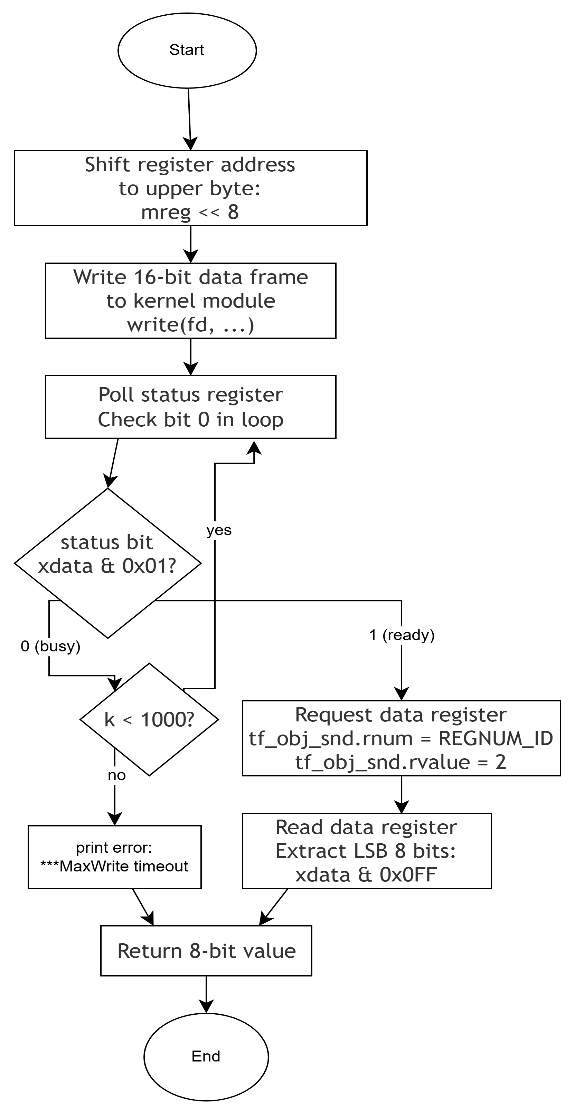
\includegraphics[scale = 1.2]{media/alin9.png}
\label{fig-alin8}
\end{figure}

when the status bit becomes 1, it indicates the read operation was successful and the result of read will be stored in the kernel module's data register.
But only LSB 8 bits of the returned value will be the data as all the MAX31865 registers are 8 bits. So the result must be masked with 0x0FF to extract the valid data: xdata \&= 0x0FF.

reading from MAX31865 with, \textbf{\texttt{readMAXSpiInterface(int fd, unsigned int mreg)}}
, where "fd" is the file descriptor and "mreg" is the register to be read.\\

Example: Reading RTD MSB register (read address: 0x01)\\
 
\texttt{msb = readMAXSpiInterface(fd, MAX31865\_REG\_RTD\_MSB);}\\
 
where \texttt{MAX31865\_REG\_RTD\_MSB = 0x01}\\

Example: Reading RTD LSB register (read address: 0x02)\\

\texttt{lsb = readMAXSpiInterface(fd, MAX31865\_REG\_RTD\_LSB);}\\

where \texttt{MAX31865\_REG\_RTD\_LSB = 0x02}. This register contains RTD bits [6:0] plus fault bit at bit 0.


\subsection{Taking Temperature Reading from MAX31865}
\begin{enumerate}
\item setting 7th, 5th, 0th bits of configuration register to 1. 
	\begin{itemize}
		\item 7th bit is for turning on MAX31865 (VBIAS), continuously keeping the sensor on will consume power so it is enabled only during measurement.
\item 5th bit is for one shot conversion - triggers a single temperature measurement.
\item 0th bit is for setting filter frequency to 50 Hz to reject power line noise.
Note: for detailed bit description see the datasheet of MAX31865 configuration register section
	\end{itemize}
	
\item Wait for 1 millisecond \texttt{(usleep(1000))} to allow the MAX31865's internal ADC to complete the resistance-to-digital conversion.

\item Read RTD MSB register (read address: 0x01) using readMAXSpiInterface(). This contains bits [14:7] of the 15-bit RTD value.
\item Then RTD LSB register (read address: 0x02) is read. This contains bits [6:0] of RTD value plus fault bit at bit 0.

\item Then MSB 8 bits and LSB 8 bits are merged using: \texttt{rtd = (msb << 8) | lsb}

\item Check if bit 0 (fault bit) is set using rtd \& 0x01. If fault is detected, read fault register (0x07) and return error code -1.

\item If no fault, right shift by 1 as 0th bit of RTD LSB reg is \texttt{fault-bit: rtd >>= 1}

\item Remaining 15-bit "result" is the RTD resistance code which can be used to calculate temperature from equation given in datasheet of MAX31856.
T(\unit{\degreeCelsius}) $\approx$ (result)/32 – 256, this equation is approximated.

\item RTD value is stored in \texttt{sample.sensor\_value} along with timestamp.

\item Sample is added to ring buffer using ringBufferAddSample(rb, \&sample) for transmission to network clients.
\end{enumerate}
\begin{figure}[H]
\centering 
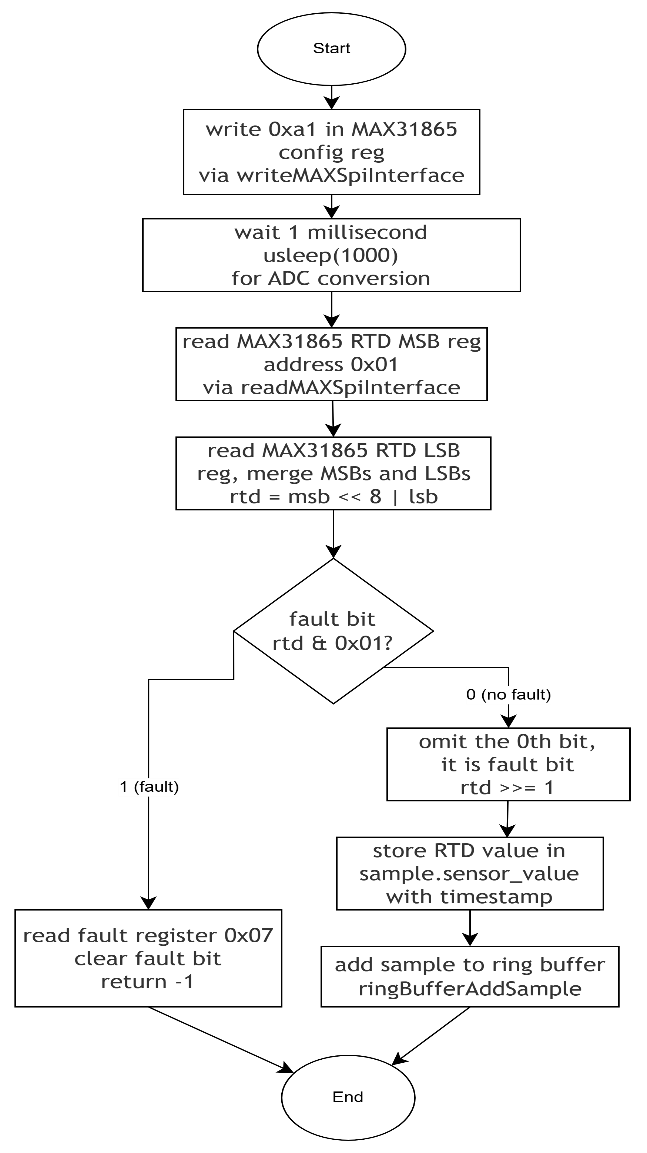
\includegraphics[scale = 1.2]{media/alin8.png}
\label{fig-alin8}
\end{figure}

\section{Shutdown Process}
The system shutdown process ensures graceful termination of all sensor operations and proper power-down of the MAX31865 temperature sensor. The shutdown sequence is coordinated through a global flag (system\_running) and involves multiple cleanup steps to ensure hardware safety and resource management.

\textbf{Shutdown Control Mechanism: }
\begin{minted}[bgcolor = lightgray, tabsize = 4, breaklines]{c}
volatile int system_running = 1;
\end{minted}

States:\\
utsystem\_running = 1 → System active, continue operation\\
system\_running = 0 → Shutdown requested, begin cleanup\\
Type: volatile ensures the variable is read from memory on every access, allowing immediate response to shutdown requests from any thread or signal handler.

\subsection{Shutdown Triggers}
The shutdown sequence can be initiated by three mechanisms:

\subsubsection{Network Command (Primary Method)}
\begin{minted}[bgcolor = lightgray, tabsize = 4, breaklines]{c}
if (strcmp(command, "SHUTDOWN") == 0) { 
printf("[NET] Shutdown command received\n"); 
system_running = 0; }
\end{minted}

\textbf{Process:}
\begin{itemize}
\item TCP client sends "SHUTDOWN\textbackslash n" command
\item Network thread sets global flag to 0
\item Sensor thread detects change and begins shutdown
\end{itemize}

\subsubsection{Signal Handler (Ctrl+C or Kill)}
\begin{minted}[bgcolor = lightgray, tabsize = 4, breaklines]{c}
void signal_handler(int signum) {
    printf("\n[MAIN] Shutting down...\n");
    system_running = 0; }
\end{minted}

\subsubsection{Error Condition}
Automatic shutdown on critical failures:

\begin{minted}[bgcolor = lightgray, tabsize = 4, breaklines]{c}
if (critical_error) {
    system_running = 0; }
\end{minted}

\textbf{Key Takeaways}
\begin{enumerate}
\item Flag-Based Control: Single global flag (system\_running) controls shutdown
\item Graceful Exit: Current operations complete before shutdown
\item Power-Down Critical: VBIAS disabled via 0x01 configuration
\item Resource Cleanup: Device file closed, thread exits cleanly
\item Fast Shutdown: Typically 1-2 ms from trigger to complete
\item Safe Restart: Clean state allows quick re-initialization
\item Power Savings: 72\% reduction in system power consumption
\end{enumerate}

\section{Reading and Writing to the Slave Registers}
\texttt{MeasObj\_struct} is used to read and write to hardware registers.
Data is written to hardware registers using the global variable \texttt{tf\_obj\_snd} of type \texttt{measObj\_struct}. Data is read from hardware registers using the global variable tf\_obj\_rcv of type measObj\_struct. The device file \texttt{(/dev/meascdd)} is used for all reading and writing operations involving hardware registers.

\subsection{Writing into the slave registers}
\begin{figure}[H]
\centering 
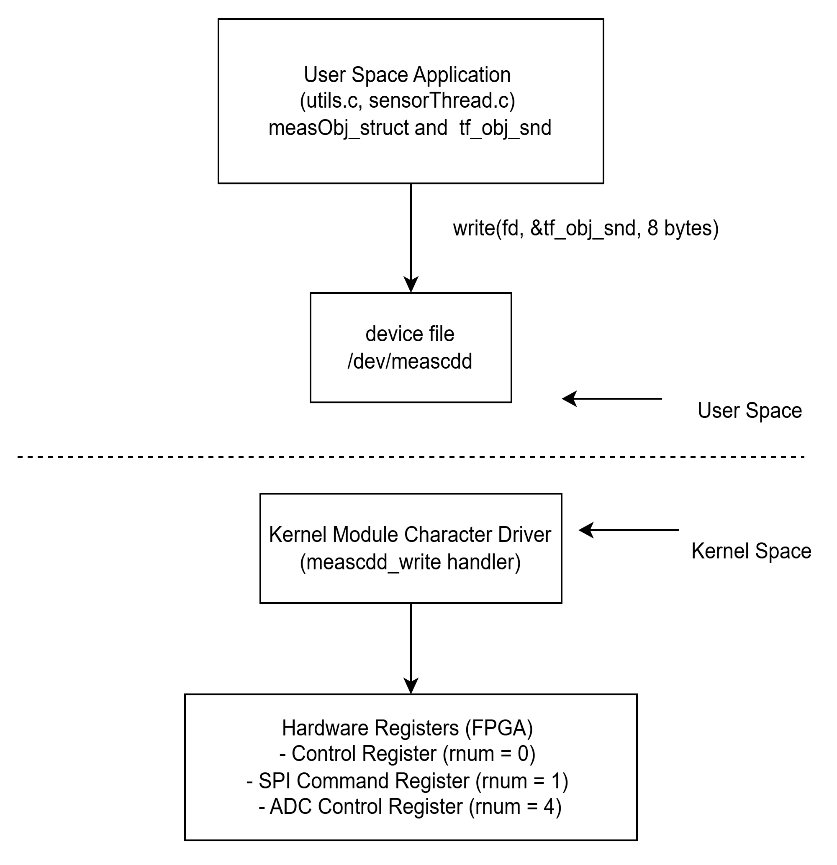
\includegraphics[scale = 1.2]{media/alin10.png}
\caption{Writing into slave registers}
\label{fig-alin10}
\end{figure}

For writing to Hardware registers 
\texttt{tf\_obj\_snd.rnum = reg;
tf\_obj\_snd.rvalue = value;}

where:

\begin{itemize}
\item "reg" is the register number (rnum selector)
\item "value" is the value to be written to the hardware register
\end{itemize}
Writing this structure to the device file via write() system call will write the "value" to the hardware registers.

\textbf{Key Points}
Kernel Module Interface: Unlike direct register access, our code uses a kernel module \texttt{(/dev/meascdd)} for hardware access. 

\begin{itemize}
\item Two-Level Addressing: 
\item First level: rnum selects the hardware register type (control, SPI, ADC)
\item Second level: For SPI operations, the 16-bit rvalue contains [address][data]
\item Status Polling: Every write operation includes status checking to ensure completion. 
\item Safety: The kernel module validates all operations before accessing hardware. 
\item Portability: Same application code works on any Linux system with the appropriate kernel module.
\end{itemize}

\begin{figure}[H]
\centering 
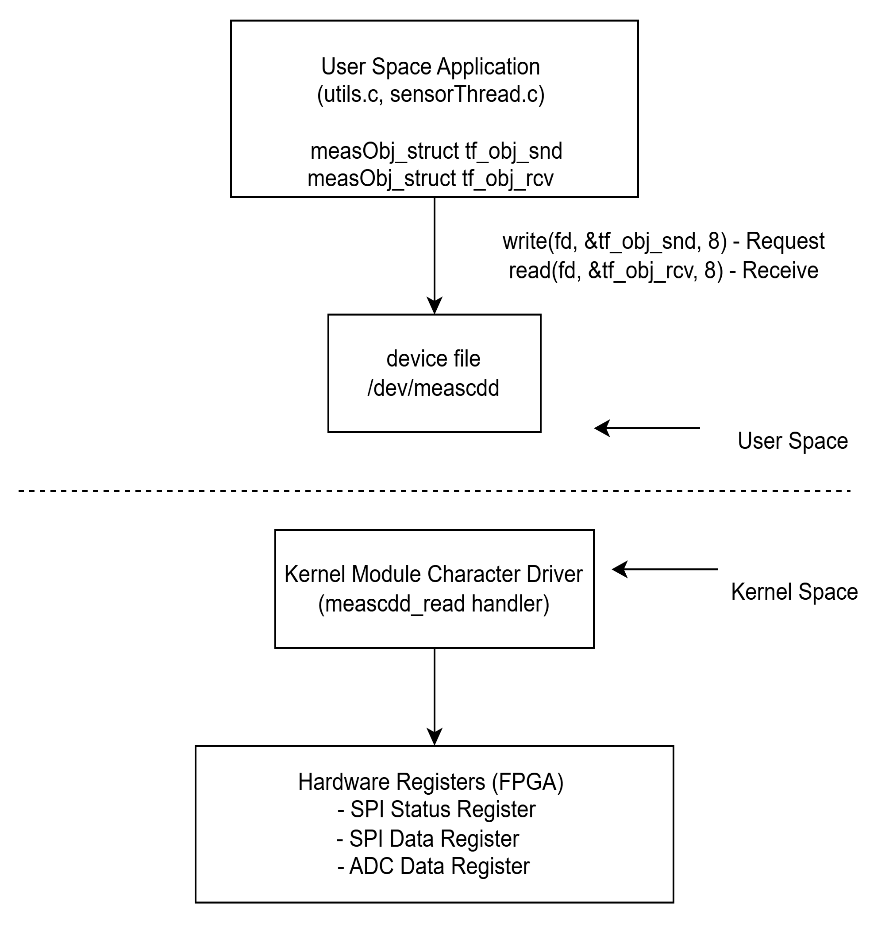
\includegraphics[scale = 1.2]{media/alin11.png}
\caption{Reading From Slave Registers}
\label{fig-alin11}
\end{figure}

For reading from hardware registers, a two-step process is used:
Step1: Send Read Command
\begin{minted}[bgcolor = lightgray, tabsize = 4, breaklines]{c}
tf_obj_snd.rnum = 1;        // SPI command register
tf_obj_snd.rvalue = mreg;   // Register address to read
write (fd, &tf_obj_snd, MEASOBJ_SIZE); 
\end{minted}

Step 2: Poll Status and Retrieve Data:
\begin{minted}[bgcolor = lightgray, tabsize = 4, breaklines]{c}
// Poll for completion

do {
    tf_obj_snd.rnum = REGNUM_ID;                          // Status register
    tf_obj_snd.rvalue = 1;                                             // Status query
    write(fd, &tf_obj_snd, MEASOBJ_SIZE);
    read(fd, &tf_obj_rcv, MEASOBJ_SIZE);
} while ((tf_obj_rcv.rvalue & 0x01) == 0);

// Retrieve data

tf_obj_snd.rnum = REGNUM_ID;
tf_obj_snd.rvalue = 2;                                                 // Data selector
write(fd, &tf_obj_snd, MEASOBJ_SIZE);
read(fd, &tf_obj_rcv, MEASOBJ_SIZE);

result = tf_obj_rcv.rvalue & 0xFF;                              // Extract 8-bit result
\end{minted}

\begin{itemize}
\item "REGNUM\_ID" (0x0FF) is the status/data register selector
\item "rvalue = 1" requests status information
\item "rvalue = 2" requests data result
\item The final result is masked to extract the 8-bit value
\end{itemize}

Reading from the device file via read() system call retrieves data from hardware registers into the tf\_obj\_rcv structure.

\textbf{Key Points}
\begin{enumerate}
\item Two-Phase Read: Read operations require sending a read command, then retrieving the result.
\item Status Polling: Every read includes status checking to wait for hardware completion.
\item Data Extraction: Results are 8-bit values extracted from 32-bit register with masking.
\item Timeout Protection: Maximum 1000 polling iterations prevents infinite loops.
\item REGNUM\_ID Modes: Special register 0x0FF provides access to status (rvalue=1) and data (rvalue=2).
\item Safe Access: Kernel module validates all operations and manages hardware access safely.
\end{enumerate}

\subsection{Comprehensive Summary and Integration}
The temperature sensing subsystem implements precision resistance temperature measurement using the MAX31865 RTD-to-digital converter. The design integrates hardware configuration, register-level SPI communication, kernel module abstraction, and structured shutdown procedures to deliver an accurate, reliable, and professionally engineered embedded solution.

The MAX31865 provides 15-bit RTD conversion with integrated fault detection and configurable filtering. Its internal architecture includes precision current sources, a differential ADC, and digital processing logic, all accessible through a structured register map. The configuration register controls bias voltage, conversion settings, and diagnostics, while data and fault registers provide measurement results and detailed error reporting.

Different RTD wiring configurations were evaluated. The 2-wire setup offers simplicity but introduces lead resistance error. The 4-wire Kelvin configuration eliminates this error entirely but increases complexity. The selected 3-wire configuration provides an effective compromise, compensating for lead resistance while maintaining practical wiring requirements for industrial applications.
Communication with the MAX31865 is performed via SPI using dedicated read and write functions. These functions construct register-specific command packets, execute transactions through a kernel module interface, and implement timeout protection to ensure robust error handling. The kernel module approach enhances system safety and portability by abstracting low-level hardware access through the /dev/meascdd device, promoting clean separation between application logic and driver-level operations.

The subsystem integrates seamlessly within a multi-sensor architecture using a thread-safe ring buffer to decouple data acquisition from network transmission. This structure ensures modularity, scalability, and reliable inter-process communication.
A structured shutdown procedure further demonstrates professional system design. The process disables sensor bias voltage to reduce power consumption, releases kernel resources, and terminates the sensor thread cleanly. This prevents hardware stress and supports stable system restarts.

Overall, the implementation reflects core embedded systems design principles: modular architecture, hardware abstraction, comprehensive error handling, and lifecycle-aware resource management. Beyond delivering accurate RTD measurement, the system establishes a scalable foundation for future extensions such as multi-sensor expansion, enhanced diagnostics, and advanced signal processing.
The result is a cohesive, maintainable, and industry-aligned embedded temperature monitoring solution suitable for professional Linux-based applications.



\section{Buttons}
\subsection{Introduction and Overview}
The hardware button monitoring system provides real-time detection and transmission of push button states from the Zedboard FPGA development platform to connected network clients. Unlike the slide switches which maintain persistent ON/OFF states, the push buttons are momentary-action devices that register as pressed only while physical pressure is applied, returning to their default released state when pressure is removed. This fundamental difference in behavior requires specific consideration in both the hardware interface design and the software implementation to accurately capture button press events and transmit them to monitoring applications.

\subsection{Physical Button Layout and Identification}
The Zedboard development board features five push buttons physically arranged in a cross pattern that facilitates directional navigation and selection operations. The center button, designated BTNC, occupies the middle position and is typically used for selection or confirmation actions. Surrounding the center button are four directional buttons: BTNU (up), BTND (down), BTNL (left), and BTNR (right), each positioned along its respective compass direction from the center. This ergonomic arrangement mirrors the layout commonly found in game controllers, remote controls, and navigation interfaces, making it intuitive for users familiar with such devices.

\begin{table}[H]
    \centering
    \caption{Push Button Descriptions}
    \begin{tabular}{|l|l|l|l|l|}
        \hline
        \textbf{Button} & \textbf{Name} & \textbf{Bit Position} & \textbf{Physical Location} & \textbf{Typical Function} \\
        \hline
        BTNC & Center & Bit 0 & Middle Of Cross & Selection/Confirmation/OK \\
        \hline
        BTND & Down   & Bit 1 & Bottom Of Cross & Navigate Down/Decrease \\
        \hline
        BTNL & Left   & Bit 2 & Left Of Cross   & Navigate Left/Previous \\
        \hline
        BTNR & Right  & Bit 3 & Right Of Cross  & Navigate Right/Next \\
        \hline
        BTNU & Up     & Bit 4 & Top Of Cross    & Navigate Up/Increase \\
        \hline
    \end{tabular}
    \caption{Hardware Button Identification}
    \label{tab:push-buttons}
\end{table}

\textbf{Explanation of Bit Positions:}
Each button is assigned a specific bit position in a 5-bit binary number. This means:

\begin{itemize}
\item When BTNC is pressed, bit 0 becomes 1
\item When BTND is pressed, bit 1 becomes 1
\item When BTNL is pressed, bit 2 becomes 1
\item When BTNR is pressed, bit 3 becomes 1
\item When BTNU is pressed, bit 4 becomes 1
\end{itemize}
When a button is released, its corresponding bit is 0. This encoding allows the hardware to represent the state of all five buttons simultaneously in just 5 bits of data.

\section{Button State Encoding System}
Since we have 5 buttons, we need 5 bits to represent all possible button states. Each bit can be either 0 or 1, where:

\begin{minted}[bgcolor = lightgray, tabsize = 4, breaklines]{text}
1 = Button is PRESSED (user is currently holding it down)
0 = Button is RELEASED (button is in its rest position)
\end{minted}

The complete 5-bit value can range from 00000 (binary) to 11111 (binary), which equals 0x00 to 0x1F in hexadecimal, or 0 to 31 in decimal.

\subsection{Example Button State Encodings}
This table shows how different button press combinations translate to binary, hexadecimal, and decimal values:

\begin{table}[H]
    \centering
    \caption{Button Press Combinations and Their Binary, Hexadecimal, and Decimal Values}
    \begin{tabular}{|l|l|l|l|l|}
        \hline
        \textbf{Buttons Pressed} & \textbf{Binary (Bit4--Bit0)} & \textbf{Hexadecimal} & \textbf{Decimal} & \textbf{Explanation} \\
        \hline
        None (all released) & 00000 & 0x00 & 0  & No buttons pressed; all bits are 0 \\
        \hline
        BTNC only           & 00001 & 0x01 & 1  & Only bit 0 is set (center button) \\
        \hline
        BTNU only           & 10000 & 0x10 & 16 & Only bit 4 is set (up button) \\
        \hline
        BTNC + BTNU         & 10001 & 0x11 & 17 & Bits 0 and 4 are set (center + up) \\
        \hline
        BTNL + BTNR         & 01100 & 0x0C & 12 & Bits 2 and 3 are set (left + right) \\
        \hline
        All 5 buttons       & 11111 & 0x1F & 31 & All bits are set (all pressed) \\
        \hline
    \end{tabular}
    \caption{Button state Encoding examples}
    \label{tab:button-combinations}
\end{table}


Detailed Explanation of Encoding Process:\\
Let's walk through how the value 0x11 (17 decimal) represents BTNC + BTNU:\\

\begin{minted}[bgcolor = lightgray, tabsize = 4, breaklines]{c}
Start with all bits as 0: 00000
BTNC is pressed: Set bit 0 to 1 -> 00001
BTNU is pressed: Set bit 4 to 1 -> 10001
Final binary: 10001
Convert to hex: 1x16¹ + 1x16⁰ = 16 + 1 = 17 decimal = 0x11 hex
Reading from right to left (LSB to MSB):
Bit 0 (rightmost): 1 = BTNC pressed 
Bit 1: 0 = BTND released
Bit 2: 0 = BTNL released
Bit 3: 0 = BTNR released
Bit 4 (leftmost): 1 = BTNU pressed 
\end{minted}

\subsection{Extracting Individual Button States from the Value}
Once you have the 5-bit button value (for example, from \texttt{readButtons()}), you need to check each bit to see which buttons are pressed. This is done using bitwise operations:
\begin{minted}[bgcolor = lightgray, tabsize = 4, breaklines]{c}
// Assume we read button_value = 0x11 (binary: 10001)
// This means BTNC and BTNU are pressed

// Extract individual button states

int is_btnc_pressed = (button_value >> 0) & 0x01;   // Bit 0 → BTNC
int is_btnd_pressed = (button_value >> 1) & 0x01;   // Bit 1 → BTND
int is_btnl_pressed = (button_value >> 2) & 0x01;   // Bit 2 → BTNL
int is_btnr_pressed = (button_value >> 3) & 0x01;   // Bit 3 → BTNR
int is_btnu_pressed = (button_value >> 4) & 0x01;   // Bit 4 → BTNU
\end{minted}
Line 1: Check BTNC (bit 0)

\begin{enumerate}
\item button\_value >> 0 shifts the value right by 0 positions (no change): 10001
\item \& 0x01 performs AND with 00001, keeping only the rightmost bit
\item Result: 00001 \& 00001 = 1, so BTNC is PRESSED
\end{enumerate}

Line 2: Check BTND (bit 1)

\begin{enumerate}
\item button\_value \>> 1 shifts right by 1: 10001 -> 01000
\item \& 0x01 keeps only the rightmost bit: 01000 \& 00001 = 0
\item Result: 0, so BTND is RELEASED
\end{enumerate}

Line 3: Check BTNL (bit 2)
\begin{enumerate}
\item button\_value \>> 2 shifts right by 2: 10001 -> 00100
\item \& 0x01 keeps only the rightmost bit: 00100 \& 00001 = 0
\item Result: 0, so BTNL is RELEASED
\end{enumerate}

Line 4: Check BTNR (bit 3)

\begin{enumerate}
\item button\_value \>> 3 shifts right by 3: 10001 -> 00010
\item \& 0x01 keeps only the rightmost bit: 00010 \& 00001 = 0
\item Result: 0, so BTNR is RELEASED
\end{enumerate}

Line 5: Check BTNU (bit 4)
\begin{enumerate}
\item button\_value \>> 4 shifts right by 3: 10001 -> 00001
\item \& 0x01 keeps only the rightmost bit: 00001 \& 00001 = 1
\item Result: 0, so BTNR is RELEASED
\end{enumerate}

Summary: With \texttt{button\_value = 0x11}, we determined that BTNC and BTNU are pressed while the other three buttons are released.

\section{Reading Button Data from Hardware}
\subsection{The \texttt{readButtons()} Function}
This function communicates with the kernel module to read the current state of all five buttons from the hardware.

\begin{minted}[bgcolor = lightgray, tabsize = 4, breaklines]{c}
unsigned int readButtons(int fd)
{
    unsigned int button_data;
    
    // Step 1: Prepare button read request

    tf_obj_snd.rnum = REGNUM_ID;     // Register selector = 0x0FF
    tf_obj_snd.rvalue = 7;            // Button selector code
    
    // Step 2: Send request to kernel module
    write(fd, &tf_obj_snd, MEASOBJ_SIZE);
    
    // Step 3: Read button states from kernel module
    read(fd, &tf_obj_rcv, MEASOBJ_SIZE);
    
    // Step 4: Extract 5-bit button data
    button_data = tf_obj_rcv.rvalue & 0x1F;
    
    // Step 5: Return the button state
      return button_data;    
}
\end{minted}

\textbf{Step 1: Prepare the Request Structure}: 
\begin{minted}[bgcolor = lightgray, tabsize = 4, breaklines]{c}
	tf_obj_snd.rnum = REGNUM_ID;     // Register selector = 0x0FF
    tf_obj_snd.rvalue = 7;            
\end{minted}

\textbf{What this does:} 
\begin{itemize}
\item \texttt{tf\_obj\_snd} is a global structure of type measObj\_struct used to send commands to the kernel module
\item \texttt{rnum = REGNUM\_ID} (which equals 0x0FF) tells the kernel module this is a special query operation
\item \texttt{rvalue = 7} specifies that we want to read button states (as opposed to switches which use rvalue = 0)
\item This is similar to filling out a request form: "What do you want?" -> "Button states (code 7)"
\end{itemize}

\textbf{Step 2: Send Request via System Call}
\begin{minted}[bgcolor = lightgray, tabsize = 4, breaklines]{c}
write(fd, &tf_obj_snd, MEASOBJ_SIZE);
\end{minted}

\textbf{What this does:}
\begin{itemize}
\item \texttt{write()} is a system call that sends data from user space to kernel space
\item fd is the file descriptor for \texttt{/dev/meascdd} device (opened earlier)
\item \texttt{\& tf\_obj\_snd} is the address of our request structure
\item \texttt{MEASOBJ\_SIZE} is 8 bytes (the size of \texttt{measObj\_struct})
\item This crosses the user-kernel boundary, triggering the kernel module's write handler
\item The kernel module receives our request and processes it
\end{itemize}

\textbf{Step 3: Read Response from Kernel}
\begin{minted}[bgcolor = lightgray, tabsize = 4, breaklines]{c}
read(fd, &tf_obj_rcv, MEASOBJ_SIZE);
\end{minted}

\textbf{What this does:}
\begin{itemize}
    \item \texttt{read()} is a system call that receives data from kernel space to user space
    \item The kernel module has already read the button GPIO register and prepared the response
    \item \texttt{\&tf\_obj\_rcv} is where the response will be stored
    \item After this call, \texttt{tf\_obj\_rcv.rvalue} contains the button state data
\end{itemize}


\textbf{Step 4: Extract and Mask Button Data}
\begin{minted}[bgcolor = lightgray, tabsize = 4, breaklines]{c}
button_data = tf_obj_rcv.rvalue & 0x1F;
\end{minted}
\textbf{What this does:}
\begin{itemize}
    \item \texttt{tf\_obj\_rcv.rvalue} is a 32-bit integer, but we only need the lower 5 bits
    \item \texttt{\& 0x1F} masks the value to keep only bits 0--4: \texttt{0x1F} = binary \texttt{00011111}
    \item This ensures we ignore any data in bits 5--31 and only keep the button information
    \item For example, if \texttt{rvalue = 0x00000511}, the mask gives us \texttt{0x11}
\end{itemize}

\textbf{Step 5: Return the Value}
\begin{minted}[bgcolor = lightgray, tabsize = 4, breaklines]{c}
return button_data;    
\end{minted}

\begin{itemize}
    \item Returns the 5-bit button state to the caller
    \item Value range: \texttt{0x00} (no buttons pressed) to \texttt{0x1F} (all buttons pressed)
\end{itemize}

\textbf{Data Flow Through the System}
\begin{enumerate}
    \item \textbf{Step 1: Physical Button Press}
    \begin{itemize}
        \item User physically presses one or more buttons on the Zedboard
        \item The mechanical switch inside each button closes, connecting a circuit
        \item This changes the voltage level on the GPIO pin from high to low (or vice versa)
    \end{itemize}

    \item \textbf{Step 2: FPGA GPIO Register}
    \begin{itemize}
        \item The FPGA continuously samples the GPIO pins connected to the buttons
        \item These 5 GPIO pin states are stored in a hardware register as a 5-bit value
        \item Example: If BTNC and BTNU are pressed, the register contains \texttt{10001} (\texttt{0x11})
    \end{itemize}

    \item \textbf{Step 3: Kernel Module}
    \begin{itemize}
        \item The Linux kernel module \texttt{/dev/meascdd} provides access to this hardware register
        \item When the application calls \texttt{readButtons()}, it communicates with this kernel module
        \item The kernel module performs memory-mapped I/O to read the FPGA register
    \end{itemize}

    \item \textbf{Step 4: readButtons() Function}
    \begin{itemize}
        \item Executes the read operation as described in section 3.1
        \item Returns the 5-bit value to the calling code
        \item Typical execution time: 5--8 microseconds
    \end{itemize}

    \item \textbf{Step 5: Create Sample Structure}
    \begin{itemize}
        \item The sensor thread receives the button value
        \item Creates a \texttt{sensor\_data\_t} structure containing:
        \begin{itemize}
            \item \texttt{sensor\_id}: Identifies this as a button sample (e.g., 2)
            \item \texttt{sensor\_value}: The 5-bit button state (\texttt{0x11})
            \item \texttt{timestamp}: Current time in microseconds
        \end{itemize}
        \item Total size: 13 bytes
    \end{itemize}

    \item \textbf{Step 6: Ring Buffer}
    \begin{itemize}
        \item The sample is added to a circular buffer (capacity: 1000 samples)
        \item This buffer is shared between the sensor thread (writer) and network thread (reader)
        \item Mutex protection ensures thread-safe access
    \end{itemize}

    \item \textbf{Step 7: Network Thread}
    \begin{itemize}
        \item Periodically (every \(\sim\)10\,ms) extracts batches of up to 100 samples
        \item Batching is more efficient than sending individual samples
        \item Mixed sensor types (temperature, switches, buttons) in same batch
    \end{itemize}

    \item \textbf{Step 8: TCP Transmission}
    \begin{itemize}
        \item The batch is sent as binary data over a TCP socket (port 8080)
        \item Each sample is exactly 13 bytes in the binary stream
        \item TCP guarantees reliable, ordered delivery
    \end{itemize}

    \item \textbf{Step 9: Client Application}
    \begin{itemize}
        \item Receives the binary stream over the network
        \item Parses 13-byte chunks as \texttt{sensor\_data\_t} structures
        \item Identifies button samples by checking \texttt{sensor\_id}
        \item Decodes the 5-bit value to determine which buttons are pressed
    \end{itemize}

\end{enumerate}


\subsection{Conclusion}
The hardware button monitoring system implements real-time detection and transmission of push button states from the Zedboard FPGA platform to network clients through a complete data acquisition pipeline. The system features five momentary-action push buttons arranged in a directional cross pattern (center, up, down, left, right), each encoded as individual bits in a 5-bit binary representation. Unlike maintained-state switches, these buttons register as pressed only during active user interaction, automatically returning to their released state when pressure is removed.

The button states are read from FPGA GPIO registers through a kernel module interface using the readButtons() function, which communicates via the /dev/meascdd character device. Each button is assigned a specific bit position (BTNC=bit 0, BTND=bit 1, BTNL=bit 2, BTNR=bit 3, BTNU=bit 4), enabling simultaneous representation of all five button states in a single 5-bit value ranging from 0x00 (all released) to 0x1F (all pressed). The system employs bitwise operations to extract individual button states and constructs 13-byte sensor\_data\_t structures containing the button value, sensor identifier, and microsecond timestamp for network transmission.

Button samples are acquired by the sensor thread according to deadline-based scheduling, stored in a thread-safe ring buffer, and transmitted to clients in binary-encoded batches over TCP connections. The complete data flow spans from physical button actuation through FPGA GPIO capture, kernel module access, application-level processing, ring buffer storage, network thread extraction, TCP transmission, to client-side parsing and display. This implementation demonstrates professional embedded systems development practices including hardware abstraction through kernel modules, efficient binary encoding, thread-safe data structures, and integration within a unified multi-sensor framework.

\newpage
\null 
\vfill
\begin{center}
\textbf{\large Ameer Muhammed (42843)}
\end{center}
\vfill
\fancyhead[L]{MNG Application (Ameer Muhammed 42843)}
\clearpage	

\chapter{MNG Application Part III}
\section{Sensor Thread Lifecycle}
\subsection{Overview of the Sensor Thread Concept}
The sensor thread constitutes the central execution entity responsible for continuous interaction with the measurement hardware on the server side of the Measurement Network Gateway. Its primary purpose is to acquire raw sensor values from the analog-to-digital converter channels and digital switch inputs, perform minimal preprocessing, and make these values available to other software components in a structured and synchronized manner.

In contrast to communication-related threads, which are inherently event-driven and dependent on external client activity, the sensor thread follows an autonomous execution model. This model ensures that sensor acquisition proceeds independently of network load, client connection state, or command frequency. Such separation is essential in embedded measurement systems, where sensor data freshness and temporal consistency must be preserved regardless of external interactions.

The lifecycle of the sensor thread spans the complete runtime of the server application, beginning with thread creation during system initialization and ending with a controlled shutdown sequence. Each phase of this lifecycle is deliberately designed to guarantee robustness, determinism, and maintainability.


\subsection{Thread Creation and Integration into the Server Process}
The creation of the sensor thread occurs during the initialization phase of the server process, after all global system resources required for concurrent execution have been successfully prepared. This includes the initialization of shared data structures, synchronization primitives, and global control flags that govern thread coordination and termination.

Creating the sensor thread early in the server startup sequence ensures that measurement data acquisition begins as soon as the system enters its operational state. This design choice decouples sensor availability from the presence of connected clients and avoids delays that could otherwise arise if acquisition were triggered only after network initialization.

From an architectural perspective, the sensor thread is created by the main application thread and registered as a long-living execution context. Once started, the thread operates continuously without requiring further intervention from the main thread, thereby reducing coupling and simplifying lifecycle management.


\begin{figure}[H]
    \centering 
    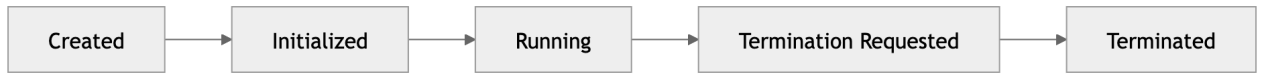
\includegraphics[width = 0.9\textwidth]{media/ameerapp1.png}
    \caption{Sensor Thread Lifecycle States}
    \label{fig-ameer1}
\end{figure}

\subsection{Initialization Phase of the Sensor Thread}
Following its creation, the sensor thread enters an initialization phase during which all thread-local resources and internal state variables are prepared. This phase establishes the foundation for safe and reliable operation throughout the runtime of the system.

Initialization includes preparing data structures used to temporarily store sensor values, verifying that utility-layer interfaces are accessible, and ensuring that the measurement device can be opened and accessed correctly. Any failure during this phase is treated as a critical condition, as continued execution without valid hardware access would lead to undefined system behavior or invalid measurement results. By performing these checks once during initialization rather than repeatedly during runtime, the implementation reduces overhead in the main execution loop and allows error conditions to be detected as early as possible.


\subsection{Transition into the Running State}
After successful initialization, the sensor thread transitions into its running state by entering a continuous execution loop. This loop constitutes the operational core of the sensor thread and remains active until a termination request is issued.

The loop-based execution model was selected deliberately over an interrupt-driven or event-based approach. While event-driven designs can be efficient under certain conditions, they often introduce additional complexity when deterministic periodic sampling is required. A loop-based model, by contrast, allows explicit control over sampling intervals, execution order, and timing behavior, which is particularly advantageous in measurement systems.

Each iteration of the loop corresponds to a single sampling cycle and is executed in a strictly sequential manner. This guarantees that all sensor values collected within one iteration represent a coherent snapshot of the system state.


\begin{figure}[H]
    \centering 
    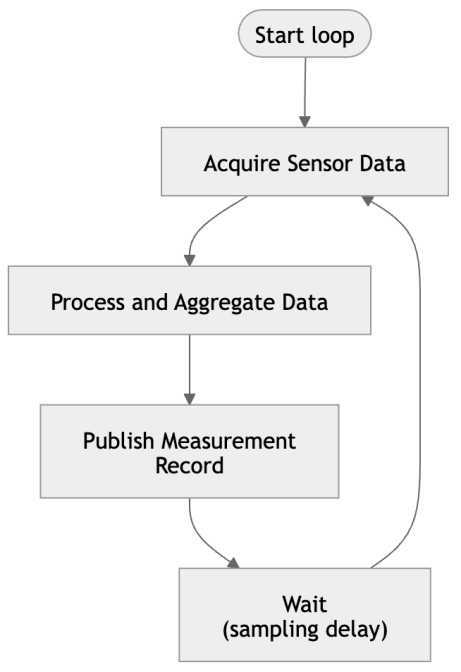
\includegraphics[scale = 0.7]{media/ameerapp3.png}
    \caption{High-Level Execution Flow of the Sensor Thread}
    \label{fig-ameer2}
\end{figure}

\subsection{Sensor Configuration Data Structure}


\begin{minted}[bgcolor = lightgray, tabsize = 4, breaklines]{c}
typedef struct
{
    sensor_id_t sid;
    uint32_t rate_hz;
    uint64_t period_us;
    uint64_t next_deadline;
    pthread_mutex_t lock;
} sensor_config_t;
\end{minted}

The behavior of the sensor thread is driven by a centralized configuration model that defines the runtime properties of each logical sensor. Each sensor is represented by a configuration structure containing its identifier, sampling rate, derived sampling period, and the next absolute deadline for acquisition. A dedicated mutex is associated with each configuration entry to allow safe runtime updates without interfering with ongoing sampling.

All sensor configurations are stored in a global array, enabling the sensor thread to iterate deterministically over all sensors within a single execution loop. This structure forms the foundation for the deadline-based scheduling mechanism described in the following sections and allows heterogeneous sensors to be managed uniformly within one thread.

\subsection{Structure of a Single Sampling Cycle}
Within each iteration of the execution loop, the sensor thread performs a fixed sequence of operations. The cycle begins with the acquisition of analog sensor values from the ADC subsystem, followed by the retrieval of digital switch states. These values are then combined into a unified measurement record representing the complete sensor state at that sampling instant.

The strict ordering of these operations is essential. By ensuring that analog and digital values are collected sequentially within the same loop iteration, the implementation avoids inconsistencies that could arise if different sensors were sampled at different times or under different system conditions.

Once all sensor values have been collected and assembled, the measurement record is handed over to a shared data structure, enabling other threads to access the data asynchronously.



\subsection{Management of Thread-Local State}
The sensor thread maintains several thread-local variables that persist across loop iterations. These variables store intermediate results such as raw ADC readings, decoded switch states, and aggregated measurement structures.

Thread-local storage plays a crucial role in simplifying concurrency control. Because these variables are not accessible to other threads, no synchronization is required during intermediate computation phases. Synchronization is only necessary when the final measurement record is published to shared memory, thereby minimizing the duration and frequency of critical sections.


\begin{table}[h]
    \centering
    \begin{tabular}{|l|l|l|}
        \hline
        \textbf{Category} & \textbf{Purpose} & \textbf{Lifetime} \\
        \hline
        Raw sensor values & Temporary storage of ADC and switch data & One loop iteration \\
        \hline
        Aggregated data & Complete measurement record & One loop iteration \\
        \hline
        Control flags & Execution and termination control & Thread lifetime \\
        \hline
    \end{tabular}
    \caption{Thread-Local State Categories in the Sensor Thread}
    \label{tab-ameer1}
\end{table}

\subsection{Interaction with Shared Resources}
From a concurrency standpoint, the sensor thread exclusively fulfills the role of a producer. It generates measurement data and publishes it to a shared buffer that is accessed by other server components. The sensor thread never consumes data from shared structures, which eliminates the possibility of circular dependencies or producer–producer conflicts.

The interaction with shared resources is deliberately confined to a narrowly defined section of the execution loop. This critical section is protected by synchronization mechanisms to guarantee atomicity and data consistency. Outside of this section, the sensor thread performs all computations without holding locks, thereby reducing contention and improving overall system responsiveness.

\begin{figure}[H]
    \centering 
    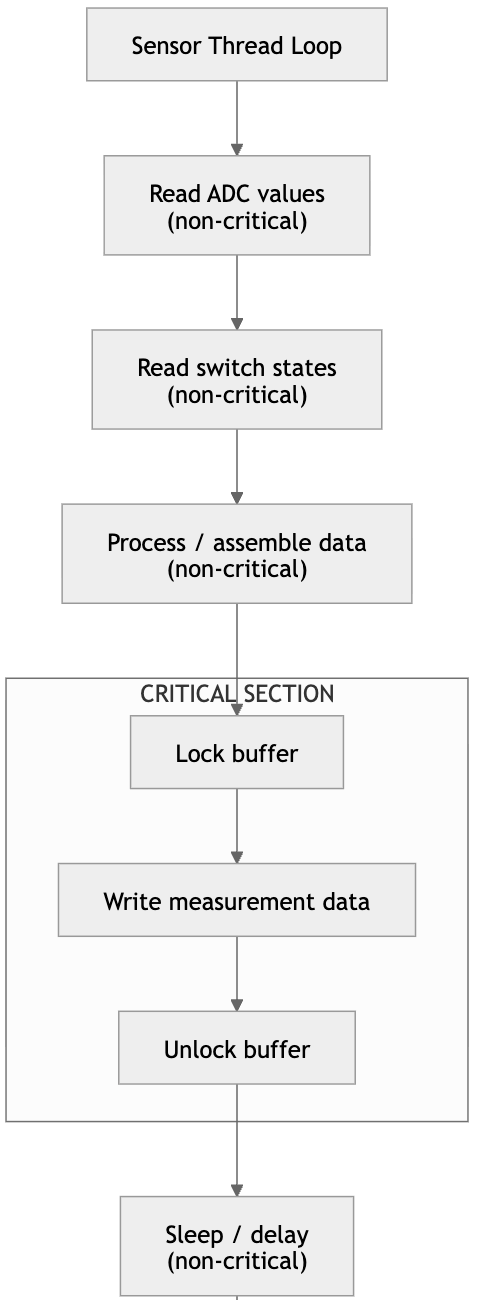
\includegraphics[scale = 0.7]{media/ameerapp4.png}
    \caption{Critical Section Placement within the Sensor Thread Loop}
    \label{fig-ameer3}
\end{figure}

\subsection{Timing Control and Sampling Period Regulation}
A key responsibility of the sensor thread is to regulate the sampling period. This is achieved by introducing an explicit delay at the end of each loop iteration. The delay duration defines the effective sampling rate and is selected based on expected sensor dynamics and system load considerations.

This approach provides a simple yet effective mechanism for controlling CPU utilization and ensuring predictable sampling behavior. While the system operates on a general-purpose Linux platform without hard real-time guarantees, the isolation of sensor acquisition into a dedicated thread allows for bounded timing variability and soft real-time behavior.


\subsection{Termination and Graceful Shutdown}
Termination of the sensor thread is initiated externally, typically as part of the overall server shutdown sequence. A shared termination flag or signal is used to inform the thread that execution should cease.

Rather than terminating immediately, the sensor thread completes its current sampling cycle before exiting the execution loop. This ensures that partially acquired data is not published and that shared resources are left in a consistent state. After exiting the loop, the thread releases any allocated resources and terminates cleanly.

\begin{figure}[H]
    \centering 
    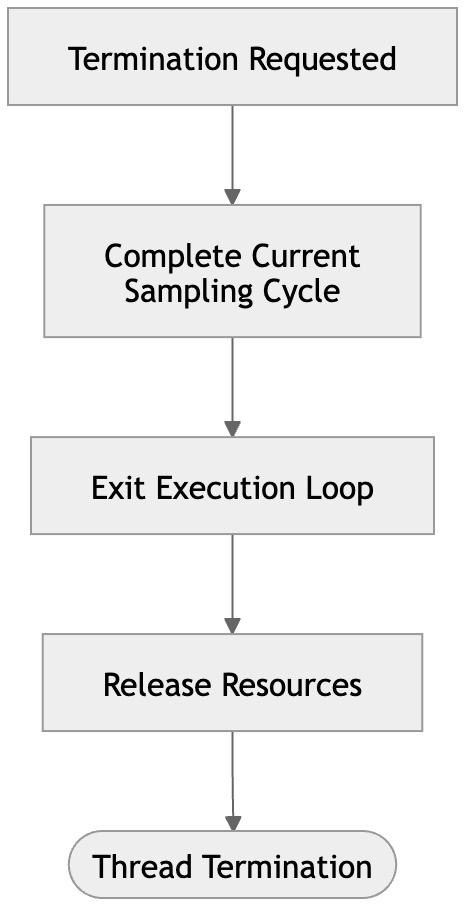
\includegraphics[scale = 0.5]{media/ameerapp5.png}
    \caption{Sensor Thread Shutdown Sequence}
    \label{fig-ameer4}
\end{figure}

\section{ADC Acquisition}
\subsection{Placement of ADC Acquisition in the Sensor Thread}
ADC acquisition is implemented entirely inside the sensor thread and is integrated into the thread’s deadline-driven main loop. The ADC logic is not isolated in a separate function; instead, it is embedded directly in the per-sensor handling switch–case structure. This design ensures that ADC acquisition follows the same scheduling and timestamping rules as all other sensors.

The ADC handling code is executed when the sensor identifier corresponds to either \texttt{adc\_zero\_sid} or \texttt{adc\_one\_sid}, as shown in the following excerpt from the sensor thread’s main loop.


\subsection{ADC-Related State Variables and Their Purpose}
Before examining the acquisition logic itself, it is important to understand the ADC-related state maintained by the sensor thread. These variables are declared at the beginning of the thread function:

\begin{minted}[bgcolor = lightgray, tabsize = 4, breaklines]{c}
static uint64_t last_adc_time = 0;
static unsigned int adc_zero_cache = 0, adc_one_cache = 0;
\end{minted}

These variables play a central role in the ADC acquisition strategy:

\begin{itemize}
    \item \texttt{last\_adc\_time} records the timestamp of the most recent ADC acquisition.
    \item \texttt{adc\_zero\_cache} and \texttt{adc\_one\_cache} store the most recently acquired ADC0 and ADC1 values.
\end{itemize}
The use of static storage duration ensures that these values persist across iterations of the sensor thread loop, allowing the ADC acquisition logic to coordinate multiple logical sensors within the same execution cycle.

\subsection{ADC Acquisition Logic in the Sensor Switch–Case}
The core ADC acquisition logic is implemented inside the switch–case statement that handles each sensor type. The following code block shows the complete ADC-related case handling exactly as implemented in \texttt{sensorThread.c:}

\begin{minted}[bgcolor = lightgray, tabsize = 4, breaklines]{c}
case adc_zero_sid:
case adc_one_sid:
    if (last_adc_time != now)
    {
        if (last_adc_time != now)
        {
            if (system_mode == MODE_SIM)
            {
                backend_read_adc(&adc_zero_cache, &adc_one_cache);
            }
            else
            {
                getADC(fd, &adc_zero_cache, &adc_one_cache);
            }

            last_adc_time = now;
        }
    }
    sample.sensor_value =
        (i == adc_zero_sid) ? adc_zero_cache : adc_one_cache;
    break;
\end{minted}
This block is the entire ADC acquisition mechanism of the server application. The design is compact but non-trivial, and each part serves a specific purpose.

\begin{minted}[bgcolor = lightgray, tabsize = 4, breaklines]{c}
if (last_adc_time != now)
\end{minted}

ensures that ADC acquisition is performed only once per scheduling instant. The variable now represents the current timestamp obtained from the high-resolution timer at the beginning of the loop iteration.

Because both ADC0 and ADC1 are processed sequentially within the same loop iteration, this condition prevents redundant ADC reads when the second logical ADC sensor is handled. Without this guard, the ADC hardware would be accessed twice per loop iteration, leading to unnecessary overhead and potential inconsistencies.

By tying ADC acquisition to the timestamp rather than to the sensor ID, the implementation guarantees that both ADC channels correspond to the same physical sampling instant.

\subsection{Simulation Mode ADC Acquisition}
Within the ADC acquisition block, the first distinction made is between simulation mode and real hardware mode:
\subsection{Timestamp-Based Synchronization of ADC Channels}
The outer condition:
\begin{minted}[bgcolor = lightgray, tabsize = 4, breaklines]{c}
if (system_mode == MODE_SIM)
{
    backend_read_adc(&adc_zero_cache, &adc_one_cache);
}
\end{minted}
In simulation mode, ADC values are generated by the \texttt{backend\_read\_adc()} function. This function provides synthetic ADC values that emulate real sensor behavior. Importantly, the simulation function writes both ADC channel values at once, matching the behavior expected from real hardware.

This design ensures that:
\begin{itemize}
    \item Simulation mode exercises the same caching, scheduling, and buffering logic as real hardware mode.

    \item Downstream components such as the ring buffer and network thread are completely unaware of whether ADC values originate from hardware or simulation.
\end{itemize}
Simulation mode therefore acts as a drop-in replacement for real ADC hardware during development, testing, and debugging.

\subsection{Hardware ADC Acquisition}
When the system is operating in real hardware mode, ADC acquisition is performed using the following call:

\begin{minted}[bgcolor = lightgray, tabsize = 4, breaklines]{c}
getADC(fd, &adc_zero_cache, &adc_one_cache);
\end{minted}
This function reads both ADC0 and ADC1 values from the hardware through the \texttt{/dev/meascdd} character device. The file descriptor fd was previously opened during sensor thread initialization and represents the user-space interface to the measurement hardware implemented in the Zynq programmable logic.

The combined ADC read approach ensures that:
\begin{itemize}
    \item Both channels are sampled during the same conversion cycle.

    \item Hardware access overhead is minimized.

    \item Channel synchronization is enforced at the acquisition level.
\end{itemize}
All time-critical operations such as SPI signaling and conversion timing are handled in hardware, while the sensor thread performs synchronous access to retrieve the completed conversion results.

\subsubsection{Measurement Device Interface for ADC Access}
Access to the ADC hardware from user space is mediated through a custom Linux character device, /dev/meascdd. The interface to this device is defined in measdev.h, which specifies the data structures and constants used for all measurement-related hardware communication. This interface forms the software–hardware boundary between the sensor thread running on the ARM processing system and the measurement logic implemented in the Zynq programmable logic.

\begin{figure}[H]
    \centering 
    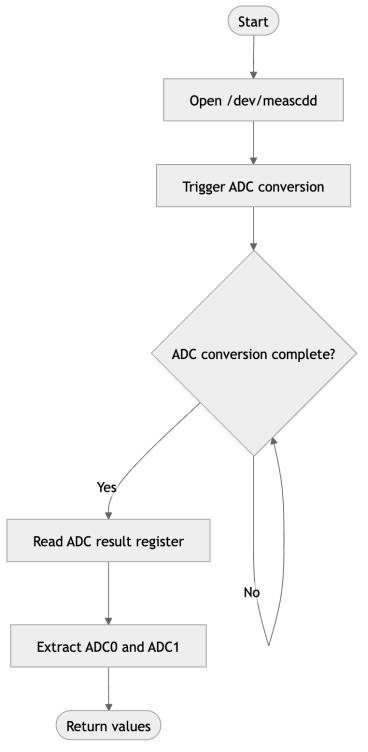
\includegraphics[scale = 1.3]{media/ameerapp6.png}
    \caption{ADC acquisition control flow}
    \label{fig-ameer5}
\end{figure}

At the core of this interface is the register object structure:
\begin{minted}[bgcolor = lightgray, tabsize = 4, breaklines]{c}
typedef struct
{
    unsigned int rnum;
    unsigned int rvalue;
} measObj_struct;
\end{minted}
Each interaction with the measurement hardware is expressed as a register-oriented transaction, where rnum identifies the target register and rvalue carries either control information or returned data. These structures are transferred atomically between user space and the kernel module using standard \texttt{read()} and \texttt{write()} system calls. The fixed size of the structure, defined by \texttt{MEASOBJ\_SIZE}, ensures deterministic and aligned communication.

The measdev interface defines symbolic identifiers such as \texttt{REGNUM\_ID} to distinguish register access operations. During ADC acquisition, these identifiers are used by the utility function getADC() to initiate a conversion, poll conversion status, and retrieve the combined ADC result register. The details of register addresses and bit-level signaling remain encapsulated within the kernel module and FPGA logic, while the user-space code operates exclusively through the abstracted register interface.

This design allows the sensor thread to remain independent of hardware-specific implementation details. The ADC acquisition logic described earlier focuses on scheduling, synchronization, and data flow, while measdev provides a consistent and reusable communication contract. The same interface is later reused for switch and push button access, reinforcing a unified hardware abstraction across the server application.

\subsection{Cache Update and Acquisition Timestamping}
After either simulation or real hardware acquisition, the ADC cache and timestamp are updated:

\begin{minted}[bgcolor = lightgray, tabsize = 4, breaklines]{c}
last_adc_time = now;
\end{minted}
This assignment marks the completion of ADC acquisition for the current loop iteration. Subsequent processing of the second ADC logical sensor within the same iteration will reuse the cached values instead of triggering a new hardware read.

This mechanism is essential for maintaining consistent behavior when multiple logical sensors share a single physical acquisition process.

\subsection{Mapping Cached ADC Values to Logical Samples}
Once ADC values are available in the cache, the sensor thread assigns the appropriate value to the current sample:

\begin{minted}[bgcolor = lightgray, tabsize = 4, breaklines]{c}
sample.sensor_value =
    (i == adc_zero_sid) ? adc_zero_cache : adc_one_cache;
\end{minted}
This line maps the physical ADC values to logical sensor samples. Each ADC channel produces its own \texttt{sensor\_data\_t} structure, containing:

\begin{itemize}
    \item A unique sensor identifier
    \item A timestamp corresponding to the acquisition instant
    \item A channel-specific digital value
\end{itemize}
Although ADC0 and ADC1 share a single acquisition operation, they are treated as independent data streams once inserted into the ring buffer.

\subsection{Integration with the Ring Buffer}
After the ADC value has been assigned, the sample is published to the shared ring buffer:

\begin{minted}[bgcolor = lightgray, tabsize = 4, breaklines]{c}
ringBufferAddSample(rb, &sample);
\end{minted}
This marks the end of ADC handling for the current sensor. From this point onward, the sensor thread no longer interacts with the ADC data. The ring buffer acts as the boundary between data acquisition and data transmission.

The network thread later consumes these samples and transmits them to connected clients, ensuring a clean producer–consumer separation between acquisition and communication.

\begin{figure}[H]
    \centering 
    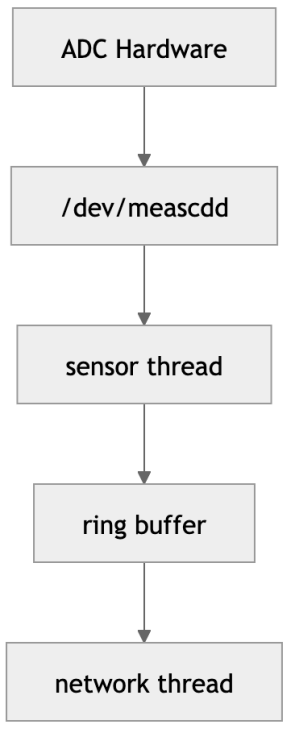
\includegraphics[scale = 0.8]{media/ameerapp7.png}
    \caption{ADC Data Flow in Sensor Thread}
    \label{fig-ameer7}
\end{figure}

\subsection{Timing Characteristics of ADC Acquisition}
ADC acquisition is synchronized with the sensor thread’s deadline-based scheduling framework. Because ADC reads occur only when the sensor deadline is reached and only once per loop iteration, the execution time overhead introduced by ADC acquisition is bounded and predictable.

This predictability is crucial in a Linux-based system where strict real-time guarantees are not available. By delegating time-critical conversion tasks to the programmable logic and limiting user-space interaction to synchronized reads, the design achieves deterministic behavior suitable for measurement applications.

\subsection{Robustness and Failure Containment}
The ADC acquisition logic is structured so that failures do not propagate beyond the sensor thread. If ADC acquisition fails or returns invalid data, only the affected sample is impacted. Other sensors continue to operate normally, and the server remains responsive.

This localized failure containment contributes to the overall robustness of the Measurement Network Gateway and ensures continued operation under adverse conditions.


\subsection{ADC Hardware Access Implementation}
While the sensor thread determines when ADC acquisition is performed, the actual mechanism for retrieving ADC values from the hardware is implemented in the utility layer. This separation of responsibilities allows the sensor thread to concentrate on scheduling, synchronization, and data flow, while low-level register access and hardware interaction are encapsulated in a dedicated module. As a result, changes to the hardware interface or register mapping can be handled locally within the utility layer without affecting higher-level logic.

The ADC hardware access is implemented by the \texttt{getADC()} function in \texttt{utils.c}. This function communicates with the Zynq programmable logic through the /dev/meascdd character device, which exposes the measurement registers implemented in the FPGA fabric to user-space software running on the processing system.

\subsubsection{Overview of the ADC Access Strategy}
The ADC subsystem provides two conversion channels, corresponding to ADC0 and ADC1. These channels are acquired together as part of a single conversion sequence, ensuring that both analog inputs are sampled at the same instant. This synchronized acquisition is particularly important when the ADC channels are used to observe related or correlated signals.

The \texttt{getADC()} function implements a structured acquisition sequence in which a conversion is first triggered in the hardware, after which the function repeatedly polls the conversion status until completion. Once the hardware indicates that valid conversion data is available, the combined ADC result register is read. This register contains the digital representations of both ADC channels, which are then separated into individual values and returned to the caller via pointer arguments.

By performing ADC acquisition in this manner, the implementation achieves deterministic behavior while keeping the user-space code simple and robust. All timing-critical operations are handled within the programmable logic, and the utility layer provides a clean, synchronous interface for higher-level software components.

\subsubsection{ADC Conversion Trigger and Status Polling}
The ADC acquisition begins by initiating a conversion through a register write:

\begin{minted}[bgcolor = lightgray, tabsize = 4, breaklines]{c}
void getADC(int fd, unsigned int *adc_zero, unsigned int *adc_one)
{
    int ccount;
    unsigned int xstatus, adc_lZero, adc1_lOne;

    tf_obj_snd.rnum = 4; // start conversion
    tf_obj_snd.rvalue = 0;
    write(fd, &tf_obj_snd, MEASOBJ_SIZE);
\end{minted}

Here, the \texttt{tf\_obj\_snd} structure is populated with a register number corresponding to the ADC control register. Writing this structure to \texttt{/dev/meascdd} triggers the programmable logic to start a conversion sequence.

Immediately after triggering the conversion, the function enters a polling loop:

\begin{minted}[bgcolor = lightgray, tabsize = 4, breaklines]{c}
    ccount = 0;
        do
        {
            ccount++;
            read(fd, &tf_obj_rcv, MEASOBJ_SIZE); // Read response from LKM
            xstatus = tf_obj_rcv.rvalue;
        } while ((xstatus == 0) && (ccount < 10000000));
\end{minted}

This loop repeatedly reads the ADC status register until the conversion is complete or a timeout threshold is reached. The polling approach ensures that the function only proceeds once valid conversion data is available, while the loop counter prevents indefinite blocking in case of hardware malfunction.

\subsubsection{Reading and Decoding ADC Result Registers}
Once conversion completion is detected, the function requests the ADC result register:

\begin{minted}[bgcolor = lightgray, tabsize = 4, breaklines]{c}
   tf_obj_snd.rnum = REGNUM_ID;
    tf_obj_snd.rvalue = 5; // ADC status register
    write(fd, &tf_obj_snd, MEASOBJ_SIZE);
    read(fd, &tf_obj_rcv, MEASOBJ_SIZE); // Read response
\end{minted}

The returned register value contains the results of both ADC channels packed into a single 32-bit word. The lower and upper portions of this word correspond to ADC0 and ADC1 respectively.

The function then extracts the individual channel values using bitwise operations:


\begin{minted}[bgcolor = lightgray, tabsize = 4, breaklines]{c}
    adc1_lOne = tf_obj_rcv.rvalue;
        adc_lZero = adc1_lOne & 0x0fff;
        adc1_lOne >>= 16;

        *adc_zero = adc_lZero;
        *adc_one = adc1_lOne;
    }
\end{minted}

\subsubsection{Interaction with the Sensor Thread}
The getADC() function is invoked by the sensor thread as part of the ADC acquisition process. During each scheduled acquisition cycle, the sensor thread calls this function to retrieve the most recent ADC conversion results from the hardware. The function returns both ADC channel values through pointer arguments, allowing the sensor thread to store the results in local cache variables. These cached values are subsequently assigned to logical sensor samples and incorporated into the standard data flow used for all sensors.

This interaction establishes a clear division of responsibilities between the sensor thread and the utility layer. The sensor thread remains agnostic to hardware-specific details and focuses solely on scheduling, synchronization, and data handling. At the same time, the utility layer encapsulates all register-level communication and hardware semantics, ensuring that any changes to ADC register mapping or access mechanisms can be confined to utils.c without affecting higher-level logic.

\subsubsection{Design Considerations and Advantages}
The ADC utility implementation provides a structured and efficient approach to hardware access within the Measurement Network Gateway. By acquiring both ADC channels in a single operation, the design guarantees synchronized dual-channel sampling while avoiding redundant hardware access. The user-space logic required to retrieve ADC data is kept intentionally minimal, reducing complexity in the sensor thread and improving maintainability.

This separation between scheduling logic and hardware access contributes to a clean architectural design in which timing-critical operations are handled within the programmable logic, while user-space software performs deterministic, synchronous access to completed conversion results. The same register-based access pattern is reused across multiple hardware interfaces, including switches and push buttons, reinforcing consistency and modularity throughout the server implementation.


\section{Switch Handling}
\subsection{Role of Switch Inputs in the Measurement Network Gateway}
Slide switches on the ZedBoard provide persistent digital input states that can be used to represent configuration settings, operating modes, or user-defined flags during system operation. Unlike push buttons, which generate momentary events, slide switches maintain a stable ON or OFF state until manually changed by the user. This makes them particularly suitable for representing long-lived system conditions that should be sampled periodically rather than edge-triggered.

In the Measurement Network Gateway, slide switches are treated as digital sensors and are integrated into the same acquisition, buffering, and transmission pipeline as analog inputs. Their states are sampled by the sensor thread at a fixed rate, timestamped, and forwarded to the ring buffer for subsequent transmission to connected clients.

\subsection{Switch Acquisition in the Sensor Thread}
Switch acquisition is implemented directly within the sensor thread’s main scheduling loop. The acquisition logic is selected based on the sensor identifier corresponding to slide switches. The complete switch-handling logic in sensorThread.c is shown below:

\begin{minted}[bgcolor = lightgray, tabsize = 4, breaklines]{c}
case sw_sid:
    if (system_mode == MODE_SIM)
        sample.sensor_value = backend_read_switches();
    else
        sample.sensor_value = readZedSwitches(fd);
    break;
\end{minted}

This code illustrates that switch handling follows the same architectural pattern as other sensors. In simulation mode, synthetic switch values are generated by a backend function, allowing the server and network stack to be tested without hardware. In real hardware mode, the sensor thread retrieves the current switch states using a dedicated utility-layer function.

The acquired switch value is stored directly in the sensor\_value field of the sample structure and is subsequently processed in the same way as all other sensor data.

\subsection{Scheduling and Timing Characteristics of Switch Sampling}
Switch sampling is governed by the same deadline-based scheduling mechanism used for all sensors. Each switch sensor entry has an associated sampling period and next-deadline timestamp stored in the sensor configuration structure. When the current time exceeds the deadline, the sensor thread reads the switch state and generates a new sample.

Because slide switch states change relatively infrequently and switch read operations are fast and non-blocking, periodic polling is an efficient and reliable acquisition strategy. The execution time of switch reads is negligible compared to analog sensor acquisition, ensuring that switch sampling does not interfere with higher-frequency sensors such as ADC channels.

\subsection{Switch Hardware Access in the Utility Layer}
The actual interaction with ZedBoard switch hardware is implemented in the utility layer within the \texttt{readZedSwitches()} function. This function abstracts the low-level register access required to retrieve the current switch states from the programmable logic.

The complete implementation of the switch access function in utils.c is shown below:
\begin{minted}[bgcolor = lightgray, tabsize = 4, breaklines]{c}
unsigned int readZedSwitches(int fd)
{
    tf_obj_snd.rnum = REGNUM_ID;
    tf_obj_snd.rvalue = 0;

    write(fd, &tf_obj_snd, MEASOBJ_SIZE);
    read(fd, &tf_obj_rcv, MEASOBJ_SIZE);

    return (tf_obj_rcv.rvalue) & 0xff;
}
\end{minted}

The function constructs a register access request using the \texttt{measObj\_struct }defined in measdev.h. The request is sent to the kernel module via a \texttt{write()} system call, and the response is retrieved using a corresponding \texttt{read()} call. The returned register value contains the digital states of multiple inputs packed into a single 32-bit word.

By masking the lower eight bits of the returned value, the function extracts the states of the slide switches and returns them as an 8-bit value to the caller. Each bit corresponds to the state of a physical switch, with a value of 1 indicating an ON position and 0 indicating OFF.

\subsection{Switch State Encoding and Interpretation}
The slide switch states are represented as a compact bit field, allowing all switch positions to be conveyed using a single integer value. Each bit in the returned value corresponds to one physical switch on the ZedBoard. This encoding enables efficient transmission and straightforward interpretation by downstream components.

\begin{table}[h]
    \centering
    \begin{tabular}{|l|l|l|}
        \hline
        \textbf{Switch Index} & \textbf{Bit Position} & \textbf{Description} \\
        \hline
        SW0 & Bit 0 & Slide switch 0 \\
        \hline
        SW1 & Bit 1 & Slide switch 1 \\
        \hline
        SW2 & Bit 2 & Slide switch 2 \\
        \hline
        SW3 & Bit 3 & Slide switch 3 \\
        \hline
        SW4 & Bit 4 & Slide switch 4 \\
        \hline
        SW5 & Bit 5 & Slide switch 5 \\
        \hline
        SW6 & Bit 6 & Slide switch 6 \\
        \hline
        SW7 & Bit 7 & Slide switch 7 \\
        \hline
    \end{tabular}
    \caption{ZedBoard Slide Switch Encoding}
\end{table}

This representation allows multiple switch states to be sampled, buffered, and transmitted as a single sensor value, minimizing overhead while preserving complete state information.


\subsection{Integration with the Measurement Device Interface }
Switch acquisition relies on the same measurement device interface (measdev) used for ADC and other sensors. The register-based communication model ensures a consistent and unified hardware abstraction across all input types. By routing switch access through the measdev interface, the server software remains insulated from hardware-specific implementation details such as GPIO wiring or FPGA register layout.

This unified interface simplifies maintenance and ensures that modifications to the hardware design or register mapping can be handled within the kernel module and utility layer without impacting the sensor thread logic.

\subsection{Data Flow from Switch Hardware to Network Transmission}
Once the switch value has been retrieved by the utility layer, it is incorporated into a \texttt{sensor\_data\_t} structure by the sensor thread along with the current timestamp and sensor identifier. The sample is then inserted into the shared ring buffer, where it becomes available to the network thread.

The network thread later retrieves buffered samples and transmits them to connected clients. From the perspective of the communication layer and the graphical user interface, switch data is handled identically to other sensor types, enabling unified visualization and analysis.

\begin{figure}[H]
    \centering 
    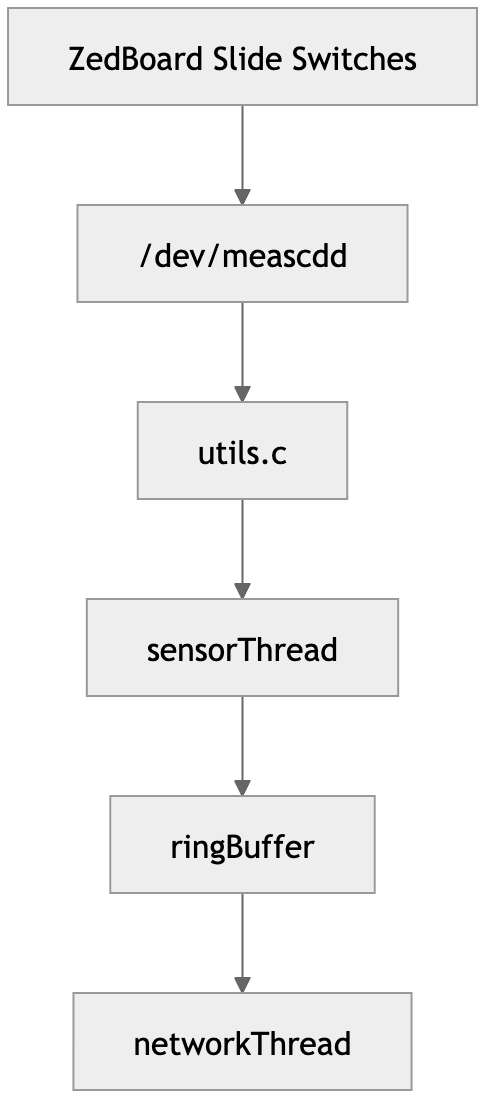
\includegraphics[scale = 0.7]{media/ameerapp8.png}
    \caption{Switch Data Flow through the Server}
    \label{fig-ameer8}
\end{figure}

\section{Utility Layer Analysis}
\subsection{Purpose of the Utility Layer}
The utility layer serves as the hardware abstraction and timing service component of the Measurement Network Gateway server. Its primary purpose is to isolate low-level hardware interaction and platform-specific functionality from the higher-level application logic implemented in the sensor thread. By centralizing these responsibilities, the utility layer enables a clear separation between what the system measures and how those measurements are obtained from the hardware.

This design reduces complexity in the sensor thread and ensures that hardware-specific details do not propagate into scheduling, buffering, or networking code.

\subsection{Abstraction of Hardware Interaction}
All direct interaction with the measurement hardware is performed through the utility layer. This includes access to ADC channels and slide switch states via the register-based interface exposed by the Linux kernel module. The sensor thread invokes utility functions to retrieve measurement values without requiring knowledge of register identifiers, bit layouts, or communication protocols.

This abstraction ensures that changes to the hardware implementation, such as modified register mappings or alternative peripherals, can be accommodated by modifying the utility layer alone. The rest of the server software remains unaffected, improving maintainability and extensibility.

\subsection{Support for Deterministic Timing}
In addition to hardware access, the utility layer provides a unified timing service based on a monotonic clock source. This timing service establishes a common reference for all sensor acquisitions and enables consistent timestamping across different sensor types.

By centralizing timing functionality, the design avoids redundant or inconsistent time calculations and ensures that all scheduling decisions made by the sensor thread are based on a stable and reliable time base. This is particularly important in a Linux environment, where system time adjustments must not affect measurement consistency.

\subsection{Consistency across Sensor Types}
Although different sensors exhibit different acquisition characteristics, the utility layer presents a consistent interaction model to the sensor thread. ADC channels, slide switches, and other inputs are accessed through uniform function calls that return ready-to-use values. The sensor thread therefore applies the same scheduling, timestamping, and buffering logic to all sensor data.

This consistency simplifies the overall system design and reinforces the modular architecture of the server. It also allows simulation mode and real hardware mode to be handled transparently at the sensor thread level.

\subsection{Interaction with Higher-Level Components}
The utility layer does not interact directly with the ring buffer or the network thread. Instead, it functions as a service provider to the sensor thread, which acts as the central coordinator of data acquisition and data flow. This strict layering prevents low-level code from becoming entangled with application-level concerns such as batching, serialization, or network transmission.

As a result, the server architecture remains cleanly layered, with well-defined responsibilities assigned to each component.

\subsection{Maintainability and Design Implications}
By encapsulating hardware access and timing services within a dedicated module, the utility layer significantly improves the maintainability of the Measurement Network Gateway. The sensor thread logic remains compact and readable, while hardware-specific complexity is localized in a single place.

This design choice supports long-term extensibility and aligns with best practices for embedded and real-time software systems, where clear abstraction boundaries are essential for reliability and scalability.


\section{Timing and Determinism}
\subsection{Motivation for Deterministic Timing in the Server}
The Measurement Network Gateway operates in a Linux user-space environment, which does not provide hard real-time guarantees. Nevertheless, predictable and repeatable timing behavior is essential for meaningful sensor data acquisition, particularly when correlating analog measurements, digital inputs, and external stimuli. The server design therefore emphasizes bounded execution time, consistent timestamping, and controlled scheduling rather than strict real-time determinism.

The timing strategy is implemented primarily within the sensor thread and is supported by the utility layer’s monotonic timing services. Together, these components provide a deterministic acquisition framework that is robust against operating system scheduling variability.

\subsection{Monotonic Time Base and Timestamp Consistency}
All timing decisions in the server are based on a monotonic clock source. During initialization, the utility layer establishes a reference time using CLOCK\_MONOTONIC, which is immune to system time adjustments such as NTP corrections or manual clock changes.

\begin{minted}[bgcolor = lightgray, tabsize = 4, breaklines]{c}
void initTimer(void)
{
    struct timespec ts;
    clock_gettime(CLOCK_MONOTONIC, &ts);
    us_startup_time = ts.tv_sec * 1000000 + ts.tv_nsec / 1000;
}
\end{minted}

Subsequent calls to getElapsedTime() return the elapsed time in microseconds relative to this startup reference. This approach ensures that all timestamps are strictly increasing and comparable across the lifetime of the server process.

\begin{minted}[bgcolor = lightgray, tabsize = 4, breaklines]{c}
uint64_t getElapsedTime(void)
{
    clock_gettime(CLOCK_MONOTONIC, &current_time);
    return (current_time.tv_sec * 1000000 + current_time.tv_nsec / 1000)
           - us_startup_time;
}
\end{minted}

By centralizing timestamp generation in the utility layer, the system avoids inconsistencies that could arise from multiple time sources or mixed clock domains.

\subsection{Deadline-Based Sensor Scheduling}
Deterministic sampling behavior is achieved through a deadline-based scheduling mechanism implemented in the sensor thread. Each sensor is associated with a sampling period and a next-deadline timestamp, which together define when acquisition should occur.

At runtime, the sensor thread continuously compares the current time against each sensor’s deadline:
\begin{minted}[bgcolor = lightgray, tabsize = 4, breaklines]{c}
if (now >= sensor_cfg[i].next_deadline)
{
    /* acquire sensor and create sample */
}
\end{minted}

This condition ensures that sensor acquisition is triggered only when the configured sampling period has elapsed. Importantly, the comparison is based on absolute time rather than relative delays, which prevents cumulative drift over long execution periods.

\subsection{Deadline Catch-Up and Overrun Handling}
After a sensor sample has been acquired, the deadline is advanced using a catch-up loop:

\begin{minted}[bgcolor = lightgray, tabsize = 4, breaklines]{c}
while (now >= sensor_cfg[i].next_deadline)
    sensor_cfg[i].next_deadline += sensor_cfg[i].period_us;
\end{minted}

This mechanism ensures that missed deadlines do not permanently shift the sampling schedule. If the sensor thread experiences a temporary delay due to operating system scheduling or transient load, the loop advances the deadline until it lies in the future. As a result, the system resumes sampling aligned with the original schedule rather than accumulating phase error.

This approach is particularly important in a Linux environment, where short scheduling delays are unavoidable but should not compromise long-term timing stability.


\subsection{Bounded Execution Time within the Sensor Thread}
Determinism in the server is further supported by bounding the execution time of the sensor thread loop. Hardware interaction is deliberately limited to synchronous register reads that complete quickly and predictably. Time-critical operations such as ADC conversion timing and SPI signaling are delegated to the programmable logic, ensuring that user-space execution time remains bounded.

Additionally, the sensor thread includes a short sleep at the end of each iteration:

\begin{minted}[bgcolor = lightgray, tabsize = 4, breaklines]{c}
usleep(50);
\end{minted}

This delay is chosen to be significantly shorter than the smallest sampling period used in the system. It reduces CPU load and prevents busy-waiting, while still allowing the thread to respond promptly to upcoming deadlines.

\subsection{Deterministic Handling of Multi-Channel Sensors}
For sensors that share a common acquisition mechanism, such as the two ADC channels, deterministic behavior is ensured by synchronizing acquisition at the timestamp level. A single acquisition operation is performed per scheduling instant, and the resulting values are reused for multiple logical sensors. This guarantees that both channels correspond to the same physical sampling time and eliminates race conditions or inconsistent readings.

By anchoring multi-channel acquisition to a single timestamp, the system maintains internal consistency even when operating under non-real-time scheduling conditions.


\subsection{Interaction with Linux Scheduling}
Although the server runs under a general-purpose Linux scheduler, its design minimizes sensitivity to scheduling jitter. Absolute-time deadlines, monotonic timestamps, and bounded execution paths ensure that short delays do not propagate into long-term timing errors.

The system does not attempt to enforce hard real-time constraints. Instead, it provides soft real-time behavior that is sufficient for measurement and monitoring applications. This design choice balances predictability with portability and simplifies deployment on standard Linux systems without requiring real-time patches.


\section{Design Alternatives}
\subsection{Rationale for Discussing Design Alternatives}
The Measurement Network Gateway server was designed with a strong emphasis on modularity, predictability, and portability within a Linux user-space environment. While the chosen architecture meets the functional and timing requirements of the project, several alternative design approaches were considered during development. This section discusses those alternatives and explains why the final design was selected over other possible implementations.

The discussion focuses on sensor acquisition timing, threading model, hardware access strategy, and operating system interaction, all of which have a direct impact on determinism and system complexity.

\subsection{Polling-Based Scheduling versus Timer-Driven Acquisition}
One alternative to the implemented deadline-based scheduling approach is a purely timer-driven design, in which each sensor acquisition is triggered by a periodic timer using functions such as usleep(period) or POSIX interval timers.

In a simple timer-driven model, each sensor would block for a fixed duration and then perform acquisition. While this approach is easy to implement, it suffers from cumulative drift when execution time varies or when the thread is preempted by the operating system. Over long runtimes, such drift can significantly distort sampling intervals.

The chosen design avoids this issue by using absolute-time deadlines based on a monotonic clock. Instead of sleeping for a fixed duration, the sensor thread compares the current time against a precomputed deadline and advances that deadline explicitly after each acquisition. This approach prevents long-term phase drift and ensures that short scheduling delays do not permanently alter sampling behavior.

\subsection{Relative Delays versus Absolute Deadlines}
Another design alternative would be to use relative delays between acquisitions, for example by sleeping for the sensor’s sampling period after each acquisition. This approach is commonly used in simpler embedded systems but is less suitable in a preemptive multitasking environment such as Linux.

In contrast, the implemented design uses absolute deadlines derived from a monotonic time base. After each acquisition, the deadline is advanced until it lies in the future, effectively compensating for any missed periods. This strategy allows the system to recover gracefully from temporary overload or scheduling jitter without accumulating timing error.

This choice directly supports the system’s determinism goals while remaining compatible with standard Linux scheduling behavior.

\subsection{Single-Threaded versus Multi-Threaded Sensor Tasks}
An alternative architectural approach would be to assign each sensor its own dedicated thread. In such a design, each thread would manage its own timing and hardware access independently. While this can simplify per-sensor logic, it introduces additional complexity in terms of thread management, synchronization, and scheduling overhead.

The chosen single sensor-thread design avoids these issues by centralizing all acquisition logic in one controlled execution context. This reduces the number of threads contending for CPU time and simplifies synchronization with shared resources such as the ring buffer. It also ensures that all sensors share a common time base and scheduling framework, which is particularly important for correlating measurements across sensor types.

\subsection{User-Space versus Kernel-Space Acquisition}
Another possible design alternative would be to perform sensor acquisition entirely within kernel space by extending the Linux device driver. This could offer tighter timing control and reduced context-switch overhead. However, kernel-space implementations are more complex to develop, harder to debug, and less portable.

The chosen user-space acquisition model strikes a balance between determinism and maintainability. Time-critical operations such as ADC conversion timing and SPI signaling are delegated to the programmable logic, while user-space software performs synchronized access to completed measurements. This separation leverages the strengths of both hardware and software without introducing unnecessary kernel complexity.

\subsection{Wall-Clock Time versus Monotonic Time Sources}
Another design decision concerns the choice of time source. Using wall-clock time functions such as \texttt{time()} or \texttt{gettimeofday()} would allow timestamps to reflect real-world time, but these functions are vulnerable to discontinuities caused by system time adjustments.

The implemented design instead relies on a monotonic clock source, ensuring that timestamps are strictly increasing and immune to external time corrections. This choice is particularly important for timing analysis, debugging, and correlating sensor data over long execution periods.

\subsection{Real-Time Linux Extensions versus Soft Real-Time Design}
The system could also have been implemented using real-time Linux extensions, such as the \texttt{PREEMPT\_RT} patch or real-time scheduling policies. While these approaches can improve timing guarantees, they introduce additional system configuration requirements and reduce portability.

The selected design adopts a soft real-time approach that achieves sufficient determinism through careful scheduling, bounded execution time, and hardware-assisted acquisition. This allows the system to run reliably on standard Linux distributions without specialized kernel support, which aligns with the educational and experimental goals of the project.

\section{Testing and Fault Analysis}
\subsection{Objectives of Testing and Validation}
The objective of testing in the Measurement Network Gateway server is to verify that the implemented acquisition architecture behaves correctly under normal operating conditions and remains stable under abnormal or degraded scenarios. Testing focuses on functional correctness, timing consistency, robustness against faults, and graceful degradation when parts of the system are stressed or unavailable.

Rather than validating individual functions in isolation, the testing strategy evaluates the complete acquisition chain, from hardware interaction through user-space processing to buffered data delivery. This approach reflects the real operational environment of the gateway and ensures that design assumptions made in earlier sections hold under practical conditions.


\subsection{Functional Validation of Sensor Acquisition}
Functional testing confirms that each sensor type produces correct and consistent data when accessed through the server. For ADC channels, known analog input signals are applied, and the resulting digital values are compared against expected ranges. Switch inputs are validated by toggling physical switches and observing corresponding changes in reported values.

Correct operation is defined not only by accurate readings, but also by correct timestamp assignment and consistent sample publication into the ring buffer. Successful functional validation demonstrates that the separation between acquisition logic, utility layer, and buffering does not introduce data corruption or misalignment.


\subsection{Timing Validation and Sampling Consistency}
Timing behavior is a critical aspect of the server design. Validation focuses on ensuring that sensor sampling adheres to the configured rates and that timestamp differences between consecutive samples remain bounded.

While Linux does not provide hard real-time guarantees, the deadline-based scheduling strategy is expected to limit jitter to acceptable levels. Timing validation is therefore performed by analyzing inter-sample intervals derived from recorded timestamps.


\subsection{Robustness Against Partial Failures}
The server is designed so that failures in one sensor path do not affect others. ADC acquisition, switch handling, and timestamp generation are independent at the logical level, even though they share the same scheduling thread. This isolation ensures that an error in one acquisition path does not block or stall the entire system.

For example, if ADC acquisition experiences increased latency due to hardware delay, switch sampling and timestamp generation continue unaffected. This robustness is particularly important in mixed-sensor environments where not all sensors have identical timing or reliability characteristics.


\subsection{Validation of Hardware–Software Boundary}
Testing also validates the interface between user-space software and the kernel-level measurement device. Register reads and writes are verified to produce consistent results, and repeated access does not lead to stale or inconsistent data.

By treating the device interface as a black box during testing, the server software is validated against realistic hardware behavior rather than idealized assumptions. This approach increases confidence that the system will behave correctly even if the underlying hardware implementation changes, as long as the register contract is preserved.

\subsection{Observability and Debug Support}
The inclusion of timestamps and structured sensor samples significantly improves observability during testing. Logged output and networked data streams allow developers to correlate sensor values with acquisition times and identify anomalies such as missed deadlines or unexpected delays.

This observability makes it possible to diagnose performance issues without invasive instrumentation or intrusive debugging techniques, which is particularly valuable in timing-sensitive systems.


\subsection{Conclusion}
This work presented the design and implementation of the server-side acquisition software for the Measurement Network Gateway. The focus was placed on sensor data acquisition, timing control, and hardware abstraction, with particular emphasis on ADC sampling and switch handling.

A deadline-based scheduling approach was employed to achieve predictable sampling behavior in a Linux user-space environment. By using a monotonic time base and absolute deadlines, the system avoids long-term drift and limits timing jitter without relying on real-time kernel extensions. Time-critical conversion and signaling tasks are delegated to programmable logic, while user-space software performs synchronized access to completed measurements.

The implementation demonstrates a clear separation of concerns between scheduling, hardware access, and data buffering. The utility layer abstracts low-level register interaction and timing functions, allowing the sensor thread to remain focused on acquisition logic and data flow. This modular structure improves readability, maintainability, and extensibility of the system.

Testing and fault analysis confirm that the system behaves robustly under normal operation and degraded conditions. Sensor acquisition remains stable in the presence of hardware delays, partial failures, and variable system load. The use of timestamped samples and buffered communication ensures that transient disturbances do not lead to data loss or system instability.

Overall, the implemented server architecture provides a reliable and extensible foundation for networked measurement systems. The design choices made in this project strike a practical balance between determinism, complexity, and portability, making the system suitable for both experimental validation and future extensions.

